%%%%%%%%%%%%%%%%%%%%%%%%%%%%%%%%%%%%%%%%%%
% Master Thesis 
% Polina Polunina
% October 2022 
%
% License:
% CC-BY-SA 4.0 -- Creative Commons Attribution-ShareAlike 4.0 International
% https://creativecommons.org/licenses/by-sa/4.0/legalcode
%%%%%%%%%%%%%%%%%%%%%%%%%%%%%%%%%%%%%%%%%%
\section{Appendix} \label{sec:appendix}
    \subsection{Galaxy histories} \label{sec:appendix:galaxy-hist}
    \subsubsection{Galaxy history links for Freyja-based branch on real datasets}
    California, US (PRJNA661613): \\
   \url{https://usegalaxy.eu/u/polina/h/sf-dataset-prjna661613-covid-19-variation-analysis-on-wgs-pe-data}\\
    Wales and Northwest England, UK (PRJEB42191): \\
    \url{https://usegalaxy.eu/u/polina/h/uk-dataset-COJAC-prjeb42191-covid-19-variation-analysis-on-artic-pe-data-1}\\
    Ontario, Canada (PRJNA824537): \\
    \url{https://usegalaxy.eu/u/polina/h/ca-dataset-freyja-prjna824537-covid-19-variation-analysis-on-artic-pe-data}\\
    Washington, US (PRJNA765346): \\
    \url{https://usegalaxy.eu/u/polina/h/us-dataset-freyja-prjna765346-covid-19-variation-analysis-on-artic-pe-data-1-1-1-1}

    \subsubsection{Galaxy history links for COJAC-based branch on real datasets}
    Wales and Northwest England, UK (PRJEB42191): \\
    \url{https://usegalaxy.eu/u/polina/h/uk-dataset-COJAC-prjeb42191-covid-19-variation-analysis-on-artic-pe-data-1}\\
    Ontario, Canada (PRJNA824537): \\
    \url{https://usegalaxy.eu/u/polina/h/ca-dataset-COJAC-prjna824537-covid-19-variation-analysis-on-artic-pe-data}\\
    Washington, US (PRJNA765346): \\
    \url{https://usegalaxy.eu/u/polina/h/us-dataset-COJAC-prjna765346-covid-19-variation-analysis-on-artic-pe-data}
    
    \subsection{Listings}
\begin{lstlisting}[language=bash, caption=macros for collection of related Freyja tool wrappers, label=list:methods:wrapper-freyja-macros]
<?xml version="1.0"?>
<macros>
    <token name="@TOOL_VERSION@">1.3.8</token>
    <token name="@VERSION_SUFFIX@">0</token>
    <token name="@PROFILE@">21.01</token>
    <xml name="biotools">
        <xrefs>
            <xref type="bio.tools">freyja</xref>
        </xrefs>
    </xml>
    <xml name="requirements">
        <requirements>
            <requirement type="package" version="@TOOL_VERSION@">freyja</requirement>
            <yield/>
        </requirements>
    </xml>
    <xml name="version">
        <version_command>freyja --version</version_command>
    </xml>
    <token name="@RUN_FREYJA_UPDATE_COMMAND@"><![CDATA[
#if $usher_update_option.choice == 'update'
    freyja update &&
#end if
]]></token>
    <token name="@PREPROCESS_VCF_INPUT@"><![CDATA[
ln -s '$variants_file' 'variants_file.vcf' &&
]]></token>
    <token name="@STANDARD_INPUT_FOR_BOOT@"><![CDATA[
#if $variants_file.ext == 'vcf'
    'variants_file.vcf'
#else
    '$variants_file'
#end if
'$depth_file'
#if $eps
    --eps '${eps}'
#end if
#if $meta
    --meta '${meta}'
#end if
$confirmedonly
]]></token>
    <token name="@CUSTOM_BARCODES_COMMAND@"><![CDATA[
#if $usher_update_option.choice == 'custom'
    --barcodes '${usher_update_option.usher_barcodes}'
#end if
]]></token>
    <token name="@DASH_COMMAND@"><![CDATA[
echo '${plot_format.plot_title}' > plot_title.txt &&
echo '${plot_format.plot_intro}' > plot_intro.txt &&
freyja dash
    #if $need_aggregation.choice == 'no'
        '$tsv_aggregated'
    #else
        'aggregated.tsv'
    #end if
    '$plot_format.csv_meta'
    plot_title.txt
    plot_intro.txt
    --output abundances_dashboard.html
]]></token>
    <token name="@PLOT_COMMAND@"><![CDATA[
freyja plot
    #if $need_aggregation.choice == 'no'
        '$tsv_aggregated'
    #else
        'aggregated.tsv'
    #end if
    --output abundances_plot.pdf
    #if $plot_format.csv_meta
        --times '${plot_format.csv_meta}'
    #end if
    #if $plot_format.interval == 'MS'
        --interval MS
    #else
        --interval D
        --windowsize 70
    #end if
]]></token>
    <token name="@PLOT_AND_DASH_COMMAND@"><![CDATA[
#if $plot_format.choice == 'dash'
    @DASH_COMMAND@
#else if $plot_format.choice == 'plot'
    freyja plot
    #if $need_aggregation.choice == 'no'
        $tsv_aggregated
    #else
        aggregated.tsv
    #end if
    --output abundances_plot.pdf
    #if $plot_format.need_metadata.choice == 'yes'
        --times '${plot_format.need_metadata.csv_meta}'
        #if $plot_format.need_metadata.interval == 'MS'
            --interval MS
        #else
            --interval D
            --windowsize 70
        #end if
    #end if
#else if $plot_format.choice == 'plot_and_dash'
    @DASH_COMMAND@ &&
    @PLOT_COMMAND@
#end if
]]></token>
    <xml name="demixing_common_options">
        <param name="depth_file" type="data" format="tabular" label="Sequencing depth file"/>
        <conditional name="usher_update_option">
            <param name="choice" type="select" label="Source of UShER barcodes data"
                   help="Freyja ships with an usher_barcodes.csv file, which the tool can access internally. Since this file gets updated rather frequently, you can also download the latest version of the file from https://github.com/andersen-lab/Freyja/raw/main/freyja/data/usher_barcodes.csv, set the dataset's datatype to csv and use it as a custom barcodes file.">
                <option value="repo" selected="true">Use data shipped with the tool (can be
                    outdated)
                </option>
                <option value="custom">Provide a custom barcodes file</option>
                <!--<option value="update">Get updated versions of the curated lineage file as well as the UShER global phylogenetic tree (can cause tool to run slowly)</option>-->
            </param>
            <when value="repo"/>
            <when value="custom">
                <param name="usher_barcodes" type="data" format="csv" label="UShER barcodes file"/>
            </when>
            <!--<when value="update" />-->
        </conditional>
        <param argument="--meta" type="data" format="json" optional="true"
               label="Custom lineage metadata file"
               help="For additional flexibility and reproducibility of analyses, a custom lineage-to-contellation mapping metadata file can be provided."/>
        <param argument="--eps" type="float" optional="true"
               label="Minimum lineage abundance tp include"
               help="e.g. 0.0001."/>
        <param argument="--confirmedonly" type="boolean" truevalue="--confirmedonly" falsevalue=""
               checked="false"
               label="Remove unconfirmed lineages from the analysis"
               help="If the UShER tree includes proposed lineages, the --confirmedonly flag removes unconfirmed lineages from the analysis."/>
    </xml>
    <token name="@HELP_HEADER@"><![CDATA[
What it does
============
Freyja is a tool to recover relative lineage abundances from mixed SARS-CoV-2 samples from a sequencing dataset (BAM aligned to the Hu-1 reference).
General information
===================
Freyja is a tool to recover relative lineage abundances from mixed SARS-CoV-2 samples from a sequencing dataset (BAM aligned to the Hu-1 reference). The method uses lineage-determining mutational "barcodes" derived from the UShER global phylogenetic tree as a basis set to solve the constrained (unit sum, non-negative) de-mixing problem.
Freyja is intended as a post-processing step after primer trimming and variant calling in iVar (Grubaugh and Gangavaparu et al., 2019). From measurements of SNV freqency and sequencing depth at each position in the genome, Freyja returns an estimate of the true lineage abundances in the sample.
]]></token>
    <xml name="citations">
        <citations>
            <citation type="doi">10.5281/zenodo.6585067</citation>
        </citations>
    </xml>
</macros>
\end{lstlisting}
\begin{lstlisting}[language=bash, caption=tool wrapper for Freyja: Call variants and get
sequencing depth information, label=list:methods:wrapper-freyja-call]
<tool id="freyja_variants" name="Freyja: Call variants"
      version="@TOOL_VERSION@+galaxy@VERSION_SUFFIX@"
      profile="@PROFILE@">
    <description>
        and get sequencing depth information
    </description>
    <macros>
        <import>macros.xml</import>
    </macros>
    <expand macro="biotools"/>
    <expand macro="requirements"/>
    <expand macro="version"/>
    <command detect_errors="exit_code"><![CDATA[
ln -s '$bam_file' 'bam_file' &&
ln -s '$ref_file' 'ref_file' &&
freyja variants 
    'bam_file'
    --variants variants 
    --depths '$depths'
    --ref 'ref_file'
    ]]></command>
    <inputs>
        <param name="bam_file" type="data" format="bam" label="BAM file"
               help="After primer trimming and alignment to reference genome."/>
        <param name="ref_file" argument="--ref" type="data" format="fasta"
               label="Reference sequence file"
               help="Note that the reference should match the fasta file used for alignment."/>
    </inputs>
    <outputs>
        <data name="variants" format="tabular" label="${tool.name} on ${on_string}: Variant call"
              from_work_dir="variants.tsv">
        </data>
        <data name="depths" format="tabular" label="${tool.name} on ${on_string}: Sequencing depth"
              from_work_dir="depths.tsv">
        </data>
    </outputs>
    <tests>
        <test expect_num_outputs="2">
            <param name="bam_file" value="test.bam"/>
            <param name="ref_file" value="NC_045512_Hu-1.fasta"/>
            <output name="variants" ftype="tabular">
                <assert_contents>
                    <has_text text="REF_CODON"/>
                    <has_text text="NC_045512.2"/>
                </assert_contents>
            </output>
            <output name="depths" ftype="tabular">
                <assert_contents>
                    <has_text text="NC_045512.2"/>
                </assert_contents>
            </output>
        </test>
    </tests>
    <help><![CDATA[
@HELP_HEADER@
Information about **freyja variants** method
============================================
The method uses both samtools and iVar. 
.. class:: warningmark
   Note that the reference should match the fasta file used for alignment. 
Outputs
=======
We get both variant call and sequencing depth information with this command.
    ]]></help>
    <expand macro="citations"/>
</tool>
\end{lstlisting}
\begin{lstlisting}[language=bash, caption=tool wrapper for Freyja: Bootstrapping method, label=list:methods:wrapper-freyja-boot]
<tool id="freyja_boot" name="Freyja: Bootstrapping" version="@TOOL_VERSION@+galaxy@VERSION_SUFFIX@"
      profile="@PROFILE@">
    <description>
        method
    </description>
    <macros>
        <import>macros.xml</import>
    </macros>
    <expand macro="biotools"/>
    <expand macro="requirements"/>
    <expand macro="version"/>
    <command detect_errors="exit_code"><![CDATA[
@RUN_FREYJA_UPDATE_COMMAND@
@PREPROCESS_VCF_INPUT@
freyja boot
    @STANDARD_INPUT_FOR_BOOT@
    --nt \${GALAXY_SLOTS:-4}
    #if $nb
        --nb $nb
    #end if
    --output_base 'boot_output'
    @CUSTOM_BARCODES_COMMAND@
    $boxplot_pdf
    ]]></command>
    <inputs>
        <param name="variants_file" type="data" format="tabular" label="Variants file"/>
        <expand macro="demixing_common_options"/>
        <param argument="--nb" type="integer" optional="true" label="Number of bootstraps"/>
        <param name="boxplot_pdf" argument="--boxplot pdf" type="boolean" truevalue="--boxplot pdf"
               falsevalue=""
               checked="false" label="Generate boxplot"/>
    </inputs>
    <outputs>
        <data name="boot_lineages" format="csv" label="${tool.name} on ${on_string}: Lineages"
              from_work_dir="boot_output_lineages.csv"/>
        <data name="boot_summarized" format="csv" label="${tool.name} on ${on_string}: Summarized"
              from_work_dir="boot_output_summarized.csv">
        </data>
        <data name="boot_lineages_plot" format="pdf"
              label="${tool.name} on ${on_string}: Lineages boxplot"
              from_work_dir="boot_output_lineages.pdf">
            <filter>boxplot_pdf</filter>
        </data>
        <data name="boot_summarized_plot" format="pdf"
              label="${tool.name} on ${on_string}: Summarized boxplot"
              from_work_dir="boot_output_summarized.pdf">
            <filter>boxplot_pdf</filter>
        </data>
    </outputs>
    <tests>
        <!-- Test 01: test tsv input files and plots -->
        <test expect_num_outputs="4">
            <conditional name="usher_update_option">
                <param name="choice" value="repo"/>
            </conditional>
            <param name="variants_file" value="variants.tsv"/>
            <param name="depth_file" value="depths.tsv"/>
            <param name="confirmedonly" value="false"/>
            <param name="nb" value="10"/>
            <param name="boxplot_pdf" value="true"/>
            <output name="boot_lineages" ftype="csv">
                <assert_contents>
                    <has_text text="B.1.617.2"/>
                </assert_contents>
            </output>
            <output name="boot_summarized" ftype="csv">
                <assert_contents>
                    <has_text text="Delta"/>
                </assert_contents>
            </output>
            <output name="boot_lineages_plot" ftype="pdf">
                <assert_contents>
                    <has_text text="Matplotlib"/>
                </assert_contents>
            </output>
            <output name="boot_summarized_plot" ftype="pdf">
                <assert_contents>
                    <has_text text="Matplotlib"/>
                </assert_contents>
            </output>
        </test>
        <!-- Test 02: test VCF input file -->
        <test expect_num_outputs="2">
            <conditional name="usher_update_option">
                <param name="choice" value="repo"/>
            </conditional>
            <param name="variants_file" value="test.vcf"/>
            <param name="depth_file" value="depths.tsv"/>
            <param name="confirmedonly" value="false"/>
            <param name="nb" value="10"/>
            <param name="boxplot_pdf" value="false"/>
            <output name="boot_lineages" ftype="csv">
                <assert_contents>
                    <has_text text="B.1.617.2"/>
                </assert_contents>
            </output>
            <output name="boot_summarized" ftype="csv">
                <assert_contents>
                    <has_text text="Delta"/>
                </assert_contents>
            </output>
        </test>
    </tests>
    <help><![CDATA[
@HELP_HEADER@
Information about **freyja boot** method
========================================
A fast bootstrapping method for freyja.
Outputs
=======
Bootstrapping method results:
1. Bootstrap lineages: the 0.025, 0.05,0.25,0.5 (median),0.75, 0.95, and 0.975 percentiles for each lineage;
2. Bootstrap summarized: WHO designated VOI/VOC
    ]]></help>
    <expand macro="citations"/>
</tool>
\end{lstlisting}
\begin{lstlisting}[language=bash, caption=tool wrapper for Freyja: Demix lineage abundances, label=list:methods:wrapper-freyja-demix]
<tool id="freyja_demix" name="Freyja: Demix" version="@TOOL_VERSION@+galaxy@VERSION_SUFFIX@"
      profile="@PROFILE@">
    <description>
        lineage abundances
    </description>
    <macros>
        <import>macros.xml</import>
    </macros>
    <expand macro="biotools"/>
    <expand macro="requirements">
        <requirement type="package" version="4.7">sed</requirement>
    </expand>
    <expand macro="version"/>
    <command detect_errors="exit_code"><![CDATA[
@RUN_FREYJA_UPDATE_COMMAND@
#if str($sample_name.source) == 'auto':
    #set $sn = $variants_in.element_identifier
#else:
    #set $sn = str($sample_name.name)
#end if
#set $in_file = $sn.replace(' ', '_') + '.' + $variants_in.ext
ln -s '$variants_in' $in_file &&
freyja demix
    '$in_file'
    '$depth_file'
    #if $eps
        --eps $eps
    #end if
    #if $meta
        --meta '$meta'
    #end if
    $confirmedonly
    @CUSTOM_BARCODES_COMMAND@
    --covcut $depth_cutoff
    --output abundances_raw.tsv &&
sed 's/$in_file/$sn/' abundances_raw.tsv > abundances.tsv
    ]]></command>
    <inputs>
        <param name="variants_in" type="data" format="tabular"
               label="Dataset with input variant calls"
               help="This can be a VCF dataset, or the tabular calls output of freayja call or ivar variants."/>
        <conditional name="sample_name">
            <param name="source" type="select" label="Set sample name"
                   help="Select autodetect to have the dataset or collection element name used as the sample name, or, for a single input dataset, provide an explicit sample name.">
                <option value="auto">Autodetect sample name</option>
                <option value="manual">Specify sample name explicitly</option>
            </param>
            <when value="auto"/>
            <when value="manual">
                <param name="name" type="text" label="Name of the sample"/>
            </when>
        </conditional>
        <expand macro="demixing_common_options"/>
        <param name="depth_cutoff" argument="--covcut" type="integer" min="0" value="10"
               multiple="true"
               label="Depth cutoff for coverage estimate"
               help="In the result file the coverage value will provide the 10x coverage estimate (percent of sites with 10 or greater reads- 10 is the default but can be modfied in this field. "/>
    </inputs>
    <outputs>
        <data name="abundances" format="tabular"
              label="${tool.name} on ${on_string}: Lineages abundances summary"
              from_work_dir="abundances.tsv"/>
    </outputs>
    <tests>
        <!-- Test 01: manual name sample -->
        <test expect_num_outputs="1">
            <param name="variants_in" value="variants.tsv"/>
            <param name="depth_file" value="depths.tsv"/>
            <conditional name="usher_update_option">
                <param name="choice" value="repo"/>
            </conditional>
            <conditional name="sample_name">
                <param name="source" value="manual"/>
                <param name="name" value="samplename"/>
            </conditional>
            <output name="abundances" ftype="tabular">
                <assert_contents>
                    <has_text text="samplename"/>
                </assert_contents>
            </output>
        </test>
        <!-- Test 02: autoname sample -->
        <test expect_num_outputs="1">
            <param name="variants_in" value="variants.tsv"/>
            <param name="depth_file" value="depths.tsv"/>
            <conditional name="usher_update_option">
                <param name="choice" value="repo"/>
            </conditional>
            <conditional name="sample_name">
                <param name="source" value="auto"/>
            </conditional>
            <output name="abundances" ftype="tabular">
                <assert_contents>
                    <has_text text="summarized"/>
                </assert_contents>
            </output>
        </test>
    </tests>
    <help><![CDATA[
@HELP_HEADER@
**Freyja demix** estimates lineage abundances in a potentially multi-lineage input sample.
Inputs
======
The tool requires as input a dataset with called variants and a dataset with genome-wide sequencing depth information.
Both types of data can be produced with *Freyja call*, but the tool accepts variant calls also in VCF format.
Note
----
For single samples it is recommended to select "Specify sample name explicitly"
under "Set sample name".
To use this tool on multiple samples in parallel, please provide two
collections in the same sample sort order - one with the variant calls, the
other one with the sequencing depths - and select "Autodetect sample name",
which will use collection element identifiers as the names of the samples.
This will produce a new collection of demixing reports that can be passed to
*Freyja: Aggregate and visualize* with sample names preserved.
Selection of multiple regular called variants and depth datasets is discouraged
since proper dataset pairing cannot be guaranteed!
Outputs
=======
The tool produces tabular output that includes the lineages detected in the sample, their corresponding abundances, and a lineage summary by constellation.
Example output:
========== ===================================================
           filename
summarized [('Delta', 0.65), ('Other', 0.25), ('Alpha', 0.1')] 
lineages   ['B.1.617.2' 'B.1.2' 'AY.6' 'Q.3']
abundances "[0.5 0.25 0.15 0.1]"
resid      3.14159
coverage   95.8
========== ===================================================
Where *summarized* denotes a sum of all lineage abundances in a particular WHO designation (i.e. B.1.617.2 and AY.6 abundances are summed in the above example), otherwise they are grouped into "Other". The *lineage* array lists the identified lineages in descending order, and *abundances* contains the corresponding abundances estimates. The value of *resid* corresponds to the residual of the weighted least absolute devation problem used to estimate lineage abundances. The *coverage* value provides the 10x coverage estimate (percent of sites with 10 or greater reads- 10 is the default but can be modfied using the *--covcut* option).
    ]]></help>
    <expand macro="citations"/>
</tool>
\end{lstlisting}
\begin{lstlisting}[language=bash, caption=tool wrapper for Freyja: Aggregate and visualize demixed results, label=list:methods:wrapper-freyja-agg]
<tool id="freyja_aggregate_plot" name="Freyja: Aggregate and visualize"
      version="@TOOL_VERSION@+galaxy@VERSION_SUFFIX@"
      profile="@PROFILE@">
    <description>
        demixed results
    </description>
    <macros>
        <import>macros.xml</import>
    </macros>
    <expand macro="biotools"/>
    <expand macro="requirements"/>
    <expand macro="version"/>
    <command detect_errors="exit_code"><![CDATA[
#if $need_aggregation.choice == 'yes'
    #set demix_dir = 'demix_outputs/'
    #set file_paths1 = []
    mkdir -p demix_outputs &&
    #for $input_file in $demix_file
        #set $file_path = $demix_dir + $input_file.element_identifier
        ln -s '$input_file' '$file_path' &&
        $file_paths1.append($file_path)
    #end for
    freyja aggregate
        '$demix_dir'
        --output aggregated.tsv
    #if $plot_format.choice != 'none'
        &&
    #end if
#end if
@PLOT_AND_DASH_COMMAND@
    ]]></command>
    <inputs>
        <conditional name="need_aggregation">
            <param name="choice" type="select"
                   label="Aggregate demixed data or provide aggregated data file?">
                <option value="yes">aggregate demixed data</option>
                <option value="no">provide aggregated data file</option>
            </param>
            <when value="yes">
                <param name="demix_file" type="data" format="tabular" multiple="true"
                       label="Lineages abundances summary file(s)" help="One file per one sample."/>
            </when>
            <when value="no">
                <param name="tsv_aggregated" type="data" format="tabular"
                       label="Provide aggregated data"/>
            </when>
        </conditional>
        <conditional name="plot_format">
            <param name="choice" type="select" label="Report(s) to generate">
                <option value="plot">non-interactive plot</option>
                <option value="dash">interactive dashboard (html)</option>
                <option value="plot_and_dash">plot and dashboard</option>
                <option value="none">no plots, just aggregated data table</option>
            </param>
            <when value="plot">
                <conditional name="need_metadata">
                    <param name="choice" type="select"
                           label="Provide a sample metadata file for plotting data over time?">
                        <option value="yes">Yes</option>
                        <option value="no">No</option>
                    </param>
                    <when value="yes">
                        <param name="csv_meta" type="data" format="csv"
                               label="Provide time(s) metadata file"
                               help="See info box below to learn more about the form of meta-file. Accepts only CSV (.csv) files"/>
                        <param name="interval" type="select" label="Choose interval" display="radio"
                               help="Used for pdf format.">
                            <option value="MS" selected="true">month bins</option>
                            <option value="D">day bins</option>
                        </param>
                    </when>
                    <when value="no"/>
                </conditional>
            </when>
            <when value="dash">
                <param name="csv_meta" type="data" format="csv"
                       label="Provide sample(s) metadata file"
                       help="See info box below to learn more about the form of meta-file. Accepts only CSV (.csv) files"/>
                <param name="plot_title" type="text" value="" optional="true" label="Title"/>
                <param name="plot_intro" type="text" value="" optional="true" label="Introduction"/>
            </when>
            <when value="plot_and_dash">
                <param name="csv_meta" type="data" format="csv"
                       label="Provide sample(s)/time(s) metadata file"
                       help="See info box below to learn more about the form of meta-file. Accepts only CSV (.csv) files"/>
                <param name="plot_title" type="text" value="" optional="true" label="Title"
                       help="Used for interactive dashboard."/>
                <param name="plot_intro" type="text" value="" optional="true" label="Introduction"
                       help="Used for interactive dashboard."/>
                <param name="interval" type="select" label="Choose interval" display="radio"
                       help="Used for pdf non-interactive plot.">
                    <option value="MS" selected="true">month bins</option>
                    <option value="D">day bins</option>
                </param>
            </when>
            <when value="none"/>
        </conditional>
    </inputs>
    <outputs>
        <!-- outputs for aggregate command -->
        <data name="aggregated" format="tabular"
              label="${tool.name} on ${on_string}: Aggregated data"
              from_work_dir="aggregated.tsv">
            <filter>need_aggregation['choice'] == 'yes'</filter>
        </data>
        <!-- outputs for dash command -->
        <data name="abundances_dashboard" format="html"
              label="${tool.name} on ${on_string}: Lineages abundances dashboard"
              from_work_dir="abundances_dashboard.html">
            <filter>plot_format['choice'] == 'dash' or plot_format['choice'] == 'plot_and_dash'
            </filter>
        </data>
        <!-- outputs for plot command -->
        <data name="abundances_plot" format="pdf"
              label="${tool.name} on ${on_string}: Lineages abundances plot"
              from_work_dir="abundances_plot.pdf">
            <filter>plot_format['choice'] == 'plot' or plot_format['choice'] == 'plot_and_dash'
            </filter>
        </data>
    </outputs>
    <tests>
        <!-- Test 01: aggregate command -->
        <test expect_num_outputs="1">
            <conditional name="need_aggregation">
                <param name="choice" value="yes"/>
                <param name="demix_file"
                       value="abundances.tsv,abundances2.tsv,abundances3.tsv,abundances4.tsv"/>
            </conditional>
            <conditional name="plot_format">
                <param name="choice" value="none"/>
            </conditional>
            <output name="aggregated" ftype="tabular">
                <assert_contents>
                    <has_text text="summarized"/>
                    <has_text text="abundances"/>
                    <has_text text="B.1.617.2"/>
                </assert_contents>
            </output>
        </test>
        <!-- Test 02: dash command -->
        <test expect_num_outputs="1">
            <conditional name="need_aggregation">
                <param name="choice" value="no"/>
                <param name="tsv_aggregated" value="bunch_of_files.tsv"/>
            </conditional>
            <conditional name="plot_format">
                <param name="choice" value="dash"/>
                <param name="csv_meta" value="csv_sample_meta.csv"/>
                <param name="plot_title" value="This is title"/>
                <param name="plot_intro" value="Local WW Dashboard"/>
            </conditional>
            <output name="abundances_dashboard" ftype="html">
                <assert_contents>
                    <has_text text="Local WW Dashboard"/>
                </assert_contents>
            </output>
        </test>
        <!-- Test 03: plot command -->
        <test expect_num_outputs="1">
            <conditional name="need_aggregation">
                <param name="choice" value="no"/>
                <param name="tsv_aggregated" value="bunch_of_files.tsv"/>
            </conditional>
            <conditional name="plot_format">
                <param name="choice" value="plot"/>
                <conditional name="need_metadata">
                    <param name="choice" value="yes"/>
                    <param name="csv_meta" value="times_metadata.csv"/>
                    <param name="interval" value="D"/>
                </conditional>
            </conditional>
            <output name="abundances_plot" ftype="pdf">
                <assert_contents>
                    <has_text text="Matplotlib"/>
                </assert_contents>
            </output>
        </test>
        <!-- Test 04: aggregate and dash commands -->
        <test expect_num_outputs="2">
            <conditional name="need_aggregation">
                <param name="choice" value="yes"/>
                <param name="demix_file" value="abundances.tsv,abundances2.tsv,abundances3.tsv"/>
            </conditional>
            <conditional name="plot_format">
                <param name="choice" value="dash"/>
                <param name="csv_meta" value="csv_sample_meta2.csv"/>
                <param name="plot_title" value="This is title"/>
                <param name="plot_intro" value="Local WW Dashboard"/>
            </conditional>
            <output name="aggregated" ftype="tabular">
                <assert_contents>
                    <has_text text="summarized"/>
                    <has_text text="abundances"/>
                    <has_text text="B.1.617.2"/>
                </assert_contents>
            </output>
            <output name="abundances_dashboard" ftype="html">
                <assert_contents>
                    <has_text text="Local WW Dashboard"/>
                </assert_contents>
            </output>
        </test>
        <!-- Test 05: aggregate and plot commands -->
        <test expect_num_outputs="2">
            <conditional name="need_aggregation">
                <param name="choice" value="yes"/>
                <param name="demix_file" value="abundances.tsv,abundances2.tsv,abundances3.tsv"/>
            </conditional>
            <conditional name="plot_format">
                <param name="choice" value="plot"/>
                <conditional name="need_metadata">
                    <param name="choice" value="yes"/>
                    <param name="csv_meta" value="csv_sample_meta2.csv"/>
                    <param name="interval" value="D"/>
                </conditional>
            </conditional>
            <output name="aggregated" ftype="tabular">
                <assert_contents>
                    <has_text text="summarized"/>
                    <has_text text="abundances"/>
                    <has_text text="B.1.617.2"/>
                </assert_contents>
            </output>
            <output name="abundances_plot" ftype="pdf">
                <assert_contents>
                    <has_text text="Matplotlib"/>
                </assert_contents>
            </output>
        </test>
        <!-- Test 06: aggregate, dash and plot commands -->
        <test expect_num_outputs="3">
            <conditional name="need_aggregation">
                <param name="choice" value="yes"/>
                <param name="demix_file" value="abundances.tsv,abundances2.tsv,abundances3.tsv"/>
            </conditional>
            <conditional name="plot_format">
                <param name="choice" value="plot_and_dash"/>
                <param name="csv_meta" value="csv_sample_meta2.csv"/>
                <param name="plot_title" value="This is title"/>
                <param name="plot_intro" value="Local WW Dashboard"/>
                <param name="interval" value="D"/>
            </conditional>
            <output name="aggregated" ftype="tabular">
                <assert_contents>
                    <has_text text="summarized"/>
                    <has_text text="abundances"/>
                    <has_text text="B.1.617.2"/>
                </assert_contents>
            </output>
            <output name="abundances_plot" ftype="pdf">
                <assert_contents>
                    <has_text text="Matplotlib"/>
                </assert_contents>
            </output>
            <output name="abundances_dashboard" ftype="html">
                <assert_contents>
                    <has_text text="Local WW Dashboard"/>
                </assert_contents>
            </output>
        </test>
    </tests>
    <help><![CDATA[
@HELP_HEADER@

Information about **freyja aggregate** method
=============================================

Method for manipulating the "demixed" output files. 

Outputs
-------

This resulting aggregated data can analyzed directly as a tsv file, or can be visualized using *freyja plot* and *freyja dash*.

Information about **freyja plot** method
========================================

Method provides a fractional abundance estimate for all aggregated samples.

A **time(s) metadata CSV file** should have this form:

*Sample,sample_collection_datetime*  

*sample_0.tsv,03/01/21*  

*sample_1.tsv,03/03/21*  
 
*sample_2.tsv,03/08/21*  

*sample_3.tsv,03/10/21*  

*sample_4.tsv,03/12/21*  

*sample_5.tsv,03/14/21*  

*sample_6.tsv,03/17/21*  

*sample_7.tsv,03/20/21*  

*sample_8.tsv,03/25/21*  

*sample_9.tsv,03/30/21*  

*sample_10.tsv,03/31/21*  

*sample_11.tsv,04/04/21*


Information about **freyja dash** method
========================================

Functionality to rapidly prepare a dashboard web page, directly from aggregated freyja output.

A **sample(s) metadata CSV file** should have this form:

*Sample,sample_collection_datetime,viral_load*  

*sample_0.tsv,03/01/21,460326*  

*sample_1.tsv,03/03/21,176645.1*  

*sample_2.tsv,03/08/21,449891.7*  

*sample_3.tsv,03/10/21,361699.5*  

*sample_4.tsv,03/12/21,658923.9*  

*sample_5.tsv,03/14/21,500432.8*  

*sample_6.tsv,03/17/21,791406.4*  

*sample_7.tsv,03/20/21,628119.9*  

*sample_8.tsv,03/25/21,810673.9*  

*sample_9.tsv,03/30/21,1263564.4*  

*sample_10.tsv,03/31/21,1627556.3*  

*sample_11.tsv,04/04/21,1528006.4*


    ]]></help>
    <expand macro="citations"/>
</tool>
\end{lstlisting}

\begin{lstlisting}[language=bash, caption=macros for collection of related Freyja tool wrappers, label=list:methods:wrapper-cojac-macros]
<?xml version="1.0"?>
<macros>
    <token name="@TOOL_VERSION@">0.2</token>
    <token name="@VERSION_SUFFIX@">0</token>
    <token name="@PROFILE@">21.01</token>
    <xml name="biotools">
        <xrefs>
            <xref type="bio.tools">cojac</xref>
        </xrefs>
    </xml>
    <xml name="requirements">
        <requirements>
            <requirement type="package" version="@TOOL_VERSION@">cojac</requirement>
            <yield/>
        </requirements>
    </xml>
    <xml name="version">
        <version_command>echo @TOOL_VERSION@</version_command>
    </xml>
    <xml name="vocdir_input">
        <conditional name="vocdir_option">
            <param name="choice" type="select"
                   label="Source of YAML files with definition of the variant of concerns"
                   help="Cojac ships with a directory with variant definitions yaml files (https://github.com/cbg-ethz/cojac/tree/master/voc), which the tool can access internally. You can also download the latest version of the yaml files from https://github.com/phe-genomics/variant_definitions and use it as a custom yamls defining the variant of concerns.">
                <option value="cache">Definitions shipped with the tool (can be outdated)</option>
                <option value="custom">From history</option>
            </param>
            <when value="cache"/>
            <when value="custom">
                <param name="voc_file" type="data" format="yaml" multiple="true"
                       label="YAML defining the variant of concern"/>
            </when>
        </conditional>
    </xml>
    <token name="@VOCDIR_COMMAND@"><![CDATA[
#if $vocdir_option.choice == 'custom'
    #set vocdir = 'voc/'
    #set file_paths1 = []
    mkdir -p voc &&
    #for $input_file in $voc_file
        #set $file_path = $vocdir + $input_file.element_identifier
        ln -s '$input_file' '$file_path' &&
        $file_paths1.append($file_path)
    #end for
#else
    DB_PATH="\$(dirname "\$(dirname "\$(which cooc-mutbamscan)")")/share/cojac" &&
    ln -s "\$DB_PATH" db &&
    #set $vocdir = 'db/voc'
#end if
]]></token>
    <token name="@HELP_HEADER@"><![CDATA[
What it does
============

The cojac package comprises a set of command-line tools to analyse co-occurrence of mutations on amplicons. It is useful, for example, for early detection of viral variants of concern (e.g. Alpha, Delta, Omicron) in environmental samples, and has been designed to scan for multiple SARS-CoV-2 variants in wastewater samples.
]]></token>
    <xml name="citations">
        <citations>
            <citation type="doi">10.1101/2021.01.08.21249379</citation>
        </citations>
    </xml>
</macros>
\end{lstlisting}
\begin{lstlisting}[language=bash, caption=tool wrapper for Cojac: mutbamscan, label=list:methods:wrapper-cojac-mutbamcsan]
<tool id="cooc_mutbamscan" name="Cojac: mutbamscan" version="@TOOL_VERSION@+galaxy@VERSION_SUFFIX@"
      profile="@PROFILE@">
    <description>
        scan an alignment file for mutation co-occurrences
    </description>
    <macros>
        <import>macros.xml</import>
    </macros>
    <expand macro="biotools"/>
    <expand macro="requirements"/>
    <expand macro="version"/>
    <command detect_errors="exit_code"><![CDATA[
ln -s '$bed_file' 'bed_file' &&
@VOCDIR_COMMAND@
#import re
#set identifier = re.sub('[^\s\w\-\\.]', '_', str($bam_file.element_identifier))
ln -s '$bam_file' ${identifier}.bam &&
ln -s '${bam_file.metadata.bam_index}' ${identifier}.bai &&
cooc-mutbamscan
    -a '${identifier}.bam'
    -b 'bed_file'
    -m '$vocdir'
    -y cooc.yaml
    -j cooc.json
    #if $amplicons_file.choice == 'build'
        -A amplicons.yaml
    #else
        -Q '$amplicons_file.in_amp'
    #end if
    -t cooc.tsv
    --cooc $cooc
    ]]></command>
    <inputs>
        <expand macro="vocdir_input"/>
        <param name="bed_file" type="data" format="bed"
               label="BED file defining the amplicons"/>
        <param name="bam_file" type="data" format="bam,cram,sam"
               label="Alignment BAM/CRAM/SAM file"/>
        <param argument="--cooc" type="integer" min="1" value="2"
               label="Minimum number of cooccurence mutations on the same amplicon"/>
        <conditional name="amplicons_file">
            <param name="choice" type="select" label="Source of amplicons YAML file">
                <option value="build">Build from BED + set of YAMLs for variants of concern</option>
                <option value="custom">From history</option>
            </param>
            <when value="build"/>
            <when value="custom">
                <param name="in_amp" type="data" format="yaml"
                       label="YAML file to query amplicons"/>
            </when>
        </conditional>
        <param name="output_files" type="select" display="checkboxes"
               multiple="true" label="Output files">
            <option value="yaml" selected="true">YAML</option>
            <option value="json">JSON</option>
            <option value="tabular">tabular</option>
        </param>
    </inputs>
    <outputs>
        <data name="cooc_yaml" format="yaml"
              label="${tool.name} on ${on_string}: Mutation cooccurrence (yaml)"
              from_work_dir="cooc.yaml">
            <filter>'yaml' in output_files</filter>
        </data>
        <data name="cooc_json" format="json"
              label="${tool.name} on ${on_string}: Mutation cooccurrence (json)"
              from_work_dir="cooc.json">
            <filter>'json' in output_files</filter>
        </data>
        <data name="cooc_tsv" format="tabular"
              label="${tool.name} on ${on_string}: Mutation cooccurrence (tabular)"
              from_work_dir="cooc.tsv">
            <filter>'tabular' in output_files</filter>
        </data>
        <data name="amplicons" format="yaml"
              label="${tool.name} on ${on_string}: Amplicons (yaml)"
              from_work_dir="amplicons.yaml">
            <filter>amplicons_file['choice'] == 'build'</filter>
        </data>
    </outputs>
    <tests>
        <!-- Test 1: build yaml for amplicons from bed and voc/ -->
        <test expect_num_outputs="4">
            <conditional name="vocdir_option">
                <param name="choice" value="custom"/>
                <param name="voc_file" value="omicron_ba1_mutations.yaml"/>
            </conditional>
            <param name="bam_file" value="tbam11.bam"/>
            <param name="bed_file" value="nCoV-2019.insert.V3.bed"/>
            <conditional name="amplicons_file">
                <param name="choice" value="build"/>
            </conditional>
            <param name="output_files" value="yaml,json,tabular"/>
            <output name="cooc_yaml" ftype="yaml">
                <assert_contents>
                    <has_text text="76_om1"/>
                    <has_text text="81_om1"/>
                </assert_contents>
            </output>
            <output name="cooc_json" ftype="json">
                <assert_contents>
                    <has_text text="76_om1"/>
                    <has_text text="81_om1"/>
                </assert_contents>
            </output>
            <output name="cooc_tsv" ftype="tabular">
                <assert_contents>
                    <has_text text="76_om1"/>
                    <has_text text="81_om1"/>
                </assert_contents>
            </output>
            <output name="amplicons" ftype="yaml">
                <assert_contents>
                    <has_text text="76_om1"/>
                    <has_text text="81_om1"/>
                </assert_contents>
            </output>
        </test>
        <!-- Test 2: supply yaml for amplicons and voc/ from cache -->
        <test expect_num_outputs="2">
            <conditional name="vocdir_option">
                <param name="choice" value="cache"/>
            </conditional>
            <param name="bam_file" value="tbam11.bam"/>
            <param name="bed_file" value="nCoV-2019.insert.V3.bed"/>
            <conditional name="amplicons_file">
                <param name="choice" value="custom"/>
                <param name="in_amp" value="amplicons111.yaml"/>
            </conditional>
            <param name="output_files" value="yaml,tabular"/>
            <output name="cooc_yaml" ftype="yaml">
                <assert_contents>
                    <has_text text="76_om1"/>
                    <has_text text="81_om1"/>
                </assert_contents>
            </output>
            <output name="cooc_tsv" ftype="tabular">
                <assert_contents>
                    <has_text text="76_om1"/>
                    <has_text text="81_om1"/>
                </assert_contents>
            </output>
        </test>
    </tests>
    <help><![CDATA[
@HELP_HEADER@

Information about **cooc-mutbamscan** method
============================================

The method scans an alignment BAM/CRAM/SAM file for mutation co-occurrences and output a JSON or YAML file.

    ]]></help>
    <expand macro="citations"/>
</tool>
\end{lstlisting}
\begin{lstlisting}[language=bash, caption=tool wrapper for Cojac: tabmut, label=list:methods:wrapper-cojac-tabmut]
<tool id="cooc_tabmut" name="Cojac: tabmut" version="@TOOL_VERSION@+galaxy@VERSION_SUFFIX@"
      profile="@PROFILE@">
    <description>
        export cooccurrence mutations as a table
    </description>
    <macros>
        <import>macros.xml</import>
    </macros>
    <expand macro="biotools"/>
    <expand macro="requirements"/>
    <expand macro="version"/>
    <command detect_errors="exit_code"><![CDATA[
#for $input_file in $cooc_file
    #set $cooc_ext = $input_file.ext
#end for
cooc-tabmut
    #if $cooc_ext == 'json'
        -j '$cooc_file'
    #else if $cooc_ext == 'yaml'
        -y '$cooc_file'
    #end if
    -o cooc-table.csv
    #if $table_orientation.choice == 'lines'
        -l
    #else if $table_orientation.choice == 'multiindex'
        -m
    #end if
    -q
    ]]></command>
    <inputs>
        <param name="cooc_file" type="data" format="json,yaml" multiple="true"
               label="Results generated by mutbamscan"/>
        <conditional name="table_orientation">
            <param name="choice" type="select" label="Output table orientation">
                <option value="columns">Column-oriented table (default)</option>
                <option value="lines">Line-oriented table</option>
                <option value="multiindex">Multi-level indexing (amplicons and counts
                    categories)
                </option>
            </param>
            <when value="columns"/>
            <when value="lines"/>
            <when value="multiindex"/>
        </conditional>
    </inputs>
    <outputs>
        <data name="table" format="csv"
              label="${tool.name} on ${on_string}: Mutation cooccurrence (CSV table)"
              from_work_dir="cooc-table.csv">
        </data>
    </outputs>
    <tests>
        <test expect_num_outputs="1">
            <param name="cooc_file" value="cooc-test111.json"/>
            <conditional name="table_orientation">
                <param name="choice" value="columns"/>
            </conditional>
            <output name="table" ftype="csv">
                <assert_contents>
                    <has_text text="A76_om1.count"/>
                    <has_text text="A76_om1.mut_oneless"/>
                </assert_contents>
            </output>
        </test>
    </tests>
    <help><![CDATA[
@HELP_HEADER@

Information about **cooc_tabmut** method
========================================

The method exports a JSON or YAML file as a CSV/TSV table for downstream analysis (e.g.: RStudio).

    ]]></help>
    <expand macro="citations"/>
</tool>
\end{lstlisting}
\begin{lstlisting}[language=bash, caption=tool wrapper for Cojac: pubmut, label=list:methods:wrapper-cojac-pubmut]
<tool id="cooc_pubmut" name="Cojac: pubmut" version="@TOOL_VERSION@+galaxy@VERSION_SUFFIX@"
      profile="@PROFILE@">
    <description>
        render a JSON or YAML file to a pretty table
    </description>
    <macros>
        <import>macros.xml</import>
    </macros>
    <expand macro="biotools"/>
    <expand macro="requirements">
        <requirement type="package" version="2.12">pandoc</requirement>
    </expand>
    <expand macro="version"/>
    <command detect_errors="exit_code"><![CDATA[
@VOCDIR_COMMAND@
#for $input_file in $cooc_file
    #set $cooc_ext = $input_file.ext
#end for
cooc-pubmut
    -m '$vocdir'
    -a '$amplicons'
    #if $cooc_ext == 'json'
        -j '$cooc_file'
    #else if $cooc_ext == 'yaml'
        -y '$cooc_file'
    #end if
    -o cooc-table.csv
    -q
    $escape
    #if $add_html
        && pandoc cooc-table.csv -o cooc-table.html
        && mkdir -p '$html.files_path'
        && cp cooc-table.html '$html.files_path'
    #end if
    ]]></command>
    <inputs>
        <expand macro="vocdir_input"/>
        <param name="amplicons" type="data" format="yaml" label="List of query amplicons"
               help="File generated by the Cojac mutbamscan tool"/>
        <param name="cooc_file" type="data" format="json,yaml" multiple="true"
               label="Results generated by mutbamscan"/>
        <param argument="--escape" type="boolean" truevalue="--escape" falsevalue=""
               checked="false" label="Use escape characters for newlines"/>
        <param name="add_html" type="boolean" checked="false"
               label="Convert CSV output table to HTML format"/>
    </inputs>
    <outputs>
        <data name="table" format="csv"
              label="${tool.name} on ${on_string}: Mutation cooccurrence (CSV table)"
              from_work_dir="cooc-table.csv">
        </data>
        <data name="html" format="html"
              label="${tool.name} on ${on_string}: Mutation cooccurrence (HTML)"
              from_work_dir="cooc-table.html">
            <filter>add_html</filter>
        </data>
    </outputs>
    <tests>
        <test expect_num_outputs="1">
            <conditional name="vocdir_option">
                <param name="choice" value="custom"/>
                <param name="voc_file" value="omicron_ba1_mutations.yaml"/>
            </conditional>
            <param name="amplicons" value="amplicons111.yaml"/>
            <param name="cooc_file" value="cooc-test111.json"/>
            <output name="table" ftype="csv">
                <assert_contents>
                    <has_text text="Amplicon 76"/>
                    <has_text text="Amplicon 81"/>
                </assert_contents>
            </output>
        </test>
    </tests>
    <help><![CDATA[
@HELP_HEADER@

Information about **cooc-pubmut** method
========================================

The method renders a JSON or YAML file to a table as in the publication.
You need to open the output CSV in a spreadsheet that understands linebreaks.

    ]]></help>
    <expand macro="citations"/>
</tool>
\end{lstlisting}







\begin{lstlisting}[language=python, caption=python script to compute the overall lineage abundances proportions of considered lineages in mock dataset for Freyja output, label=list:methods:freyja-vocs-abundances]
#create a dataframe of lineage abundances for freyja
df_fr = (pd.read_csv("data/galaxy-data/freyja_aggregated_data.tsv", sep='\t')
             # remove columns
             .drop((['summarized','resid', 'coverage']), axis=1))
            
df_fr.insert(3,'fr_delta', 0.0)
df_fr.insert(4,'fr_ba1', 0.0)
df_fr.insert(5,'fr_ba2', 0.0)
df_fr.insert(6,'fr_other', 0.0)

#compute the overall lineage abundances proportions for delta, BA1, BA2, and other for Freyja output
delta = ['B.1.617.2', 'AY']
fr_dic = {}

for ind in df_fr.index:
    ab_d = 0.0
    ab_ba1 = 0.0
    ab_ba2 = 0.0
    ab_o = 0.0
    l = df_fr['lineages'][ind]
    a = df_fr['abundances'][ind]
    dic = dict(zip(l.split(), [float(i) for i in a.split()]))
    for i, j in dic.items():
        if any(x in i for x in delta):
            ab_d += j
            x = {'delta': ab_d}
            fr_dic.update(x)
            df_fr['fr_delta'][ind] = ab_d
        elif 'BA.1' in i:
            ab_ba1 += j
            x = {'ba1': ab_ba1}
            fr_dic.update(x)
            df_fr['fr_ba1'][ind] = ab_ba1
        elif 'BA.2' in i:
            ab_ba2 += j
            x = {'ba2': ab_ba2}
            fr_dic.update(x)
            df_fr['fr_ba2'][ind] = ab_ba2
        else:
            ab_o += j
            x = {'other': ab_o}
            fr_dic.update(x)
            df_fr['fr_other'][ind] = ab_o
        
df_fr = df_fr.drop((['lineages','abundances']), axis=1)
\end{lstlisting}
    \subsection{Further figures}
        \subsubsection{Existing Galaxy workflows that were not changed} \label{sec:appendix:figures:wfs}
        Other existing Galaxy workflows for SARS-CoV-2 clinical data surveillanve that were not taken as a basis for improvement and repurposing in this thesis are presented in \cref{fig:further:ont-wf} and \cref{fig:further:illumina-wf}.
        \begin{landscape}
        \centering\vspace*{\fill}
        \begin{figure}[ht!]
        	\centering
            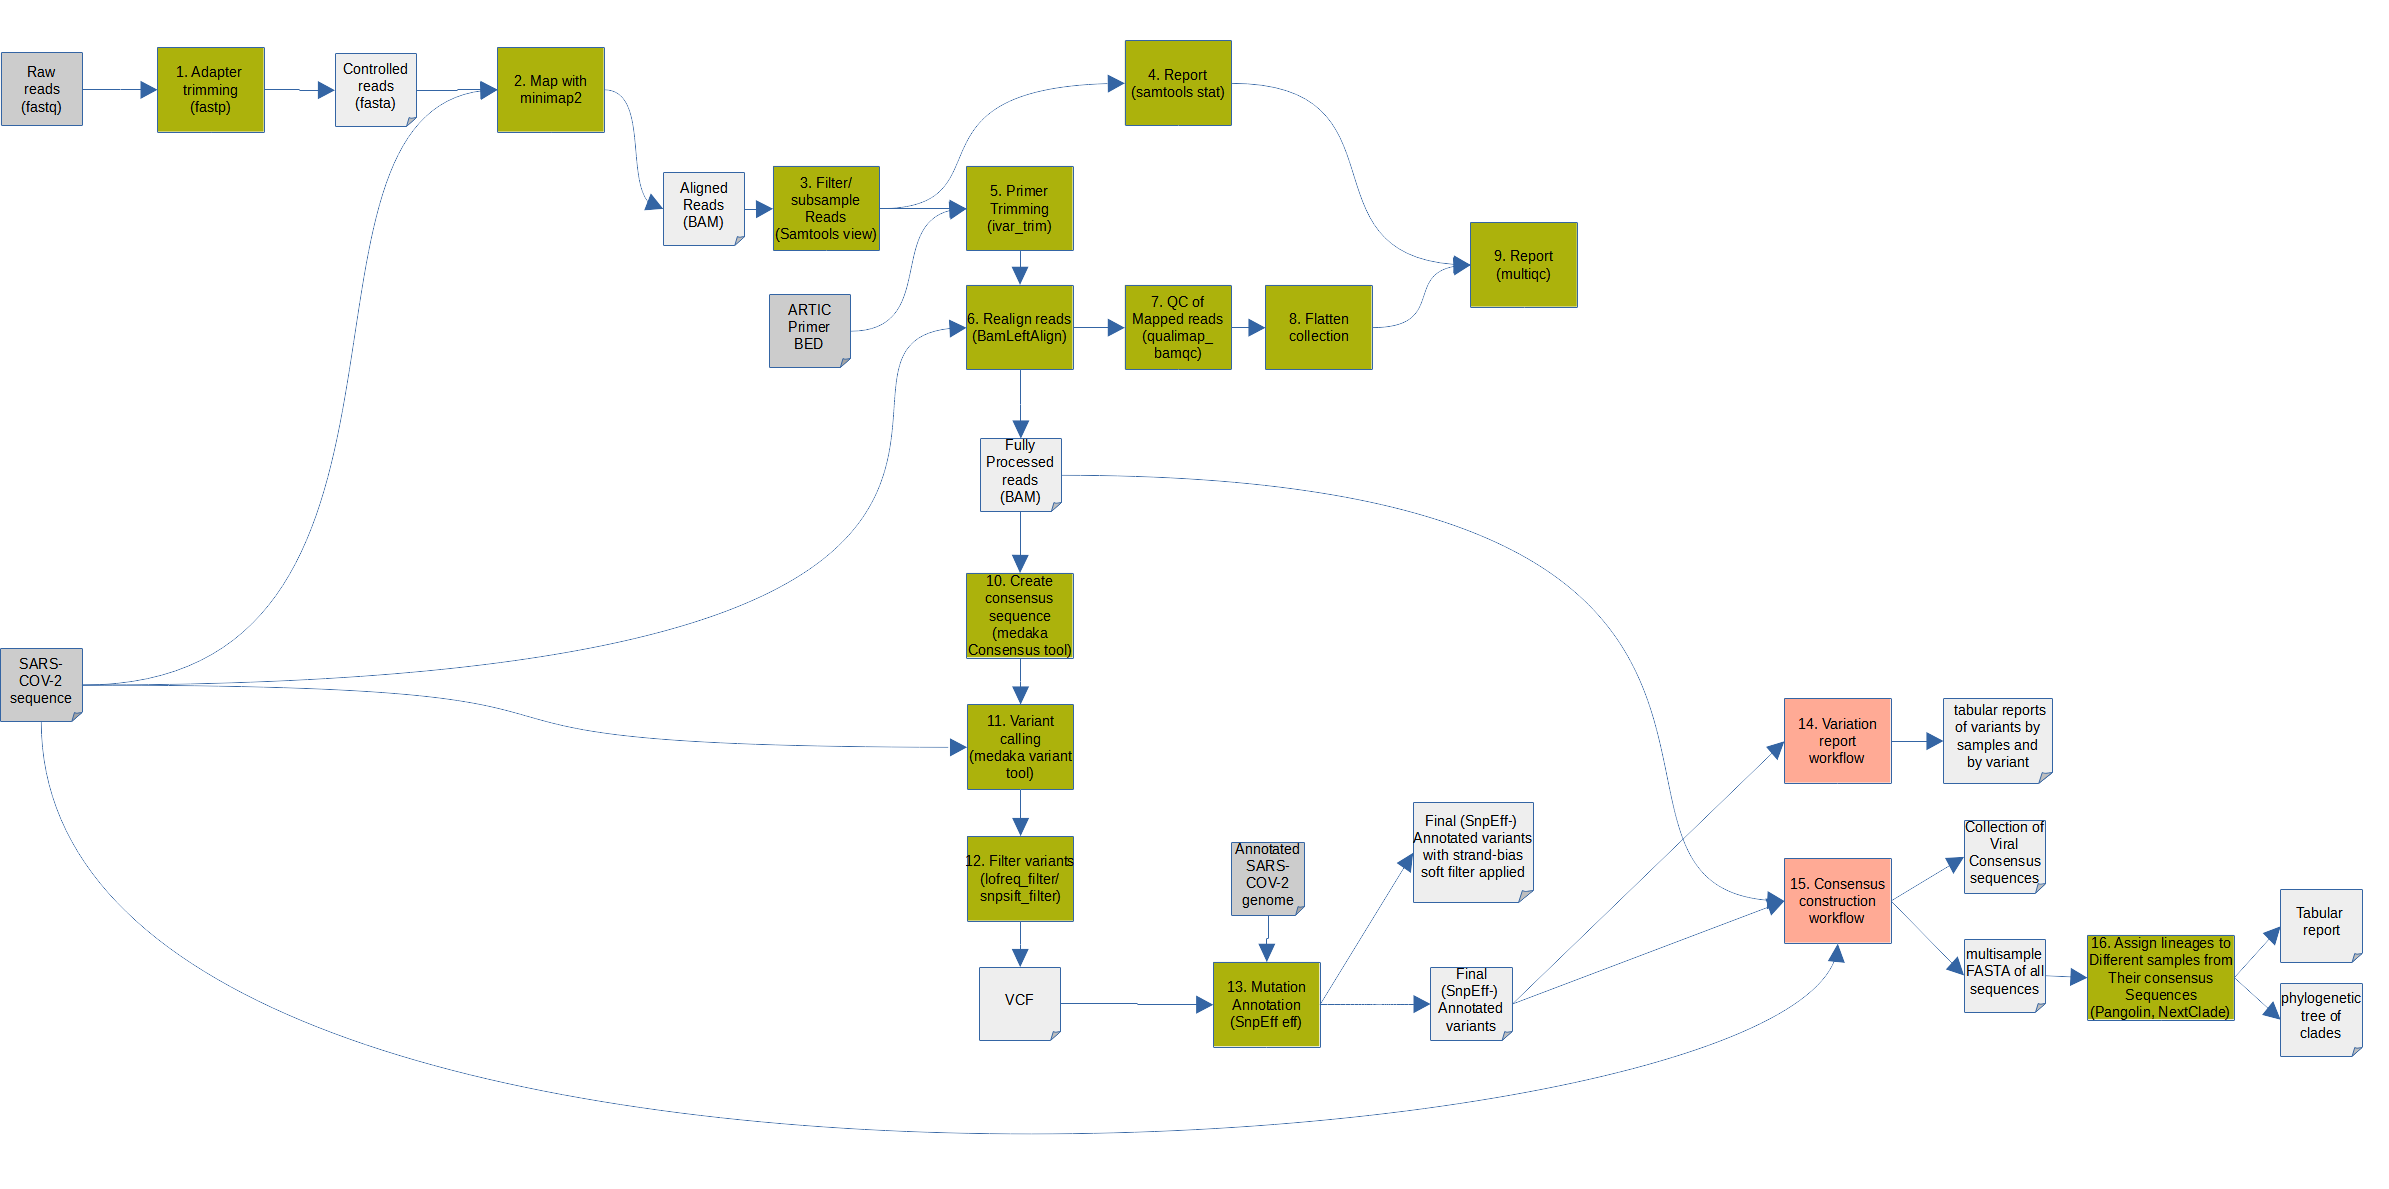
\includegraphics[width=1.4\textwidth]{figures/further/further-ont-wf.png}
            \captionof{figure}{One of four existing Galaxy workflow for SARS-CoV-2 clinical data surveillance for single-end reads data extracted with amplicon-based technique and sequenced with Nanopore sequencing approach.}
            \label{fig:further:ont-wf}
        \end{figure}
        \begin{figure}[ht!]
        	\centering
            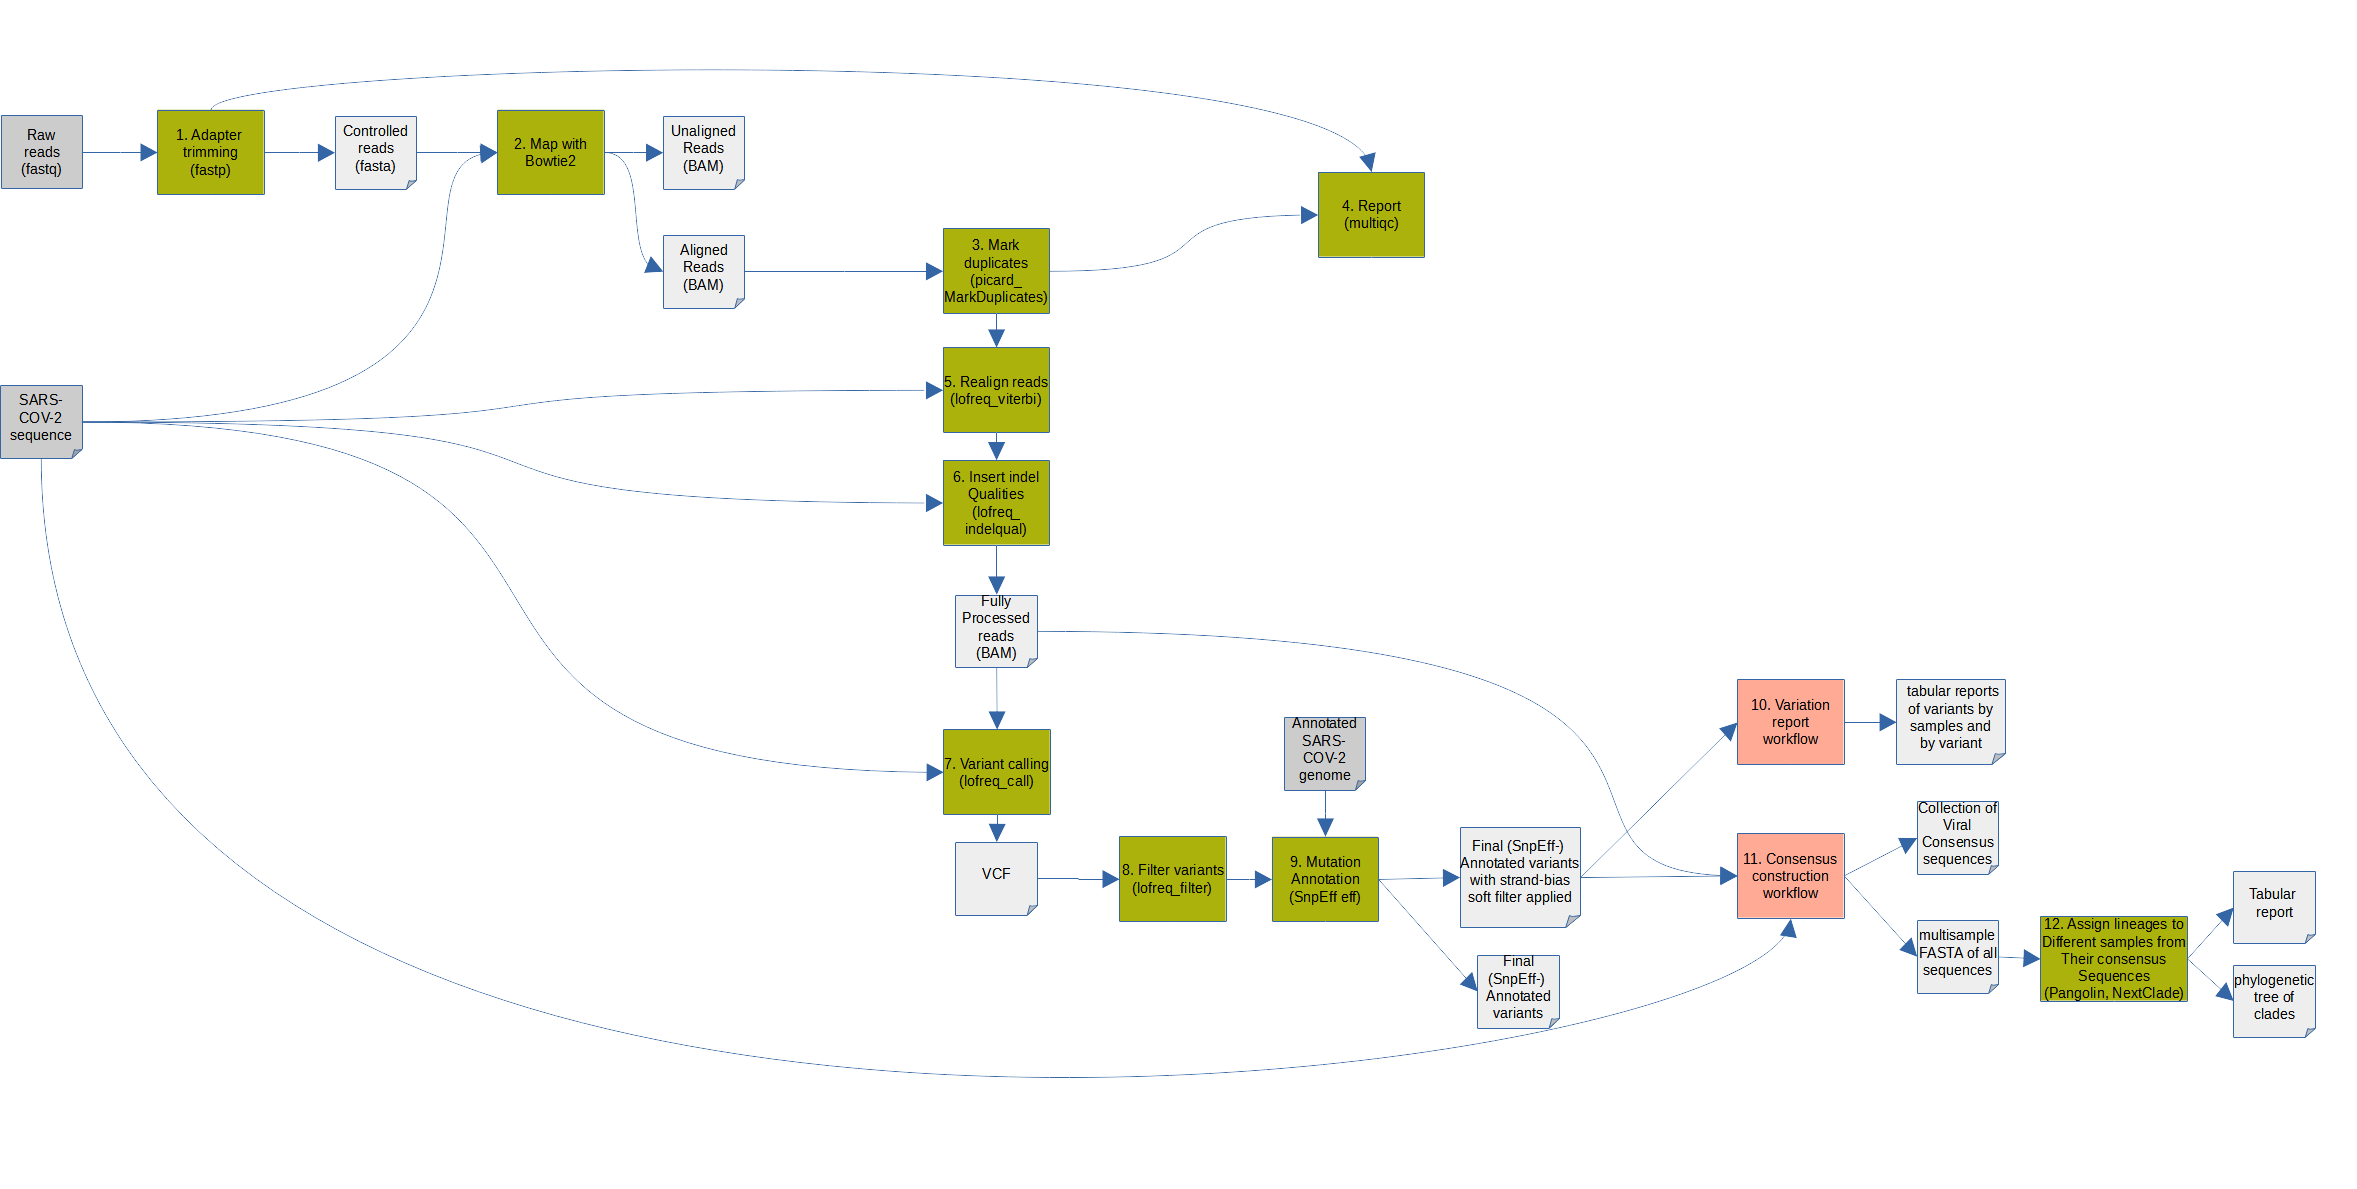
\includegraphics[width=1.4\textwidth]{figures/further/further-illumina-wf.png}
            \captionof{figure}{One of four existing Galaxy workflow for SARS-CoV-2 clinical data surveillance for single-end reads data extracted with metatranscriptomic-based technique and sequenced with Illumina sequencing approach.}
            \label{fig:further:illumina-wf}
        \end{figure}
        \vfill
        \end{landscape}
        
        \subsubsection{Parallel coordinates} 
        \paragraph{Parallel coordinates for all mock samples} \label{sec:appendix:figures:parallel-all}
        \Cref{fig:further:parallel-delta-all}, \cref{fig:further:parallel-ba1-all} and \cref{fig:further:parallel-ba2-all} depict parallel coordinates for all samples considering only detection of Delta, BA.1, and BA.2 lineage respectively by Freyja and COJAC.
        \begin{figure}[H]
        	\centering
            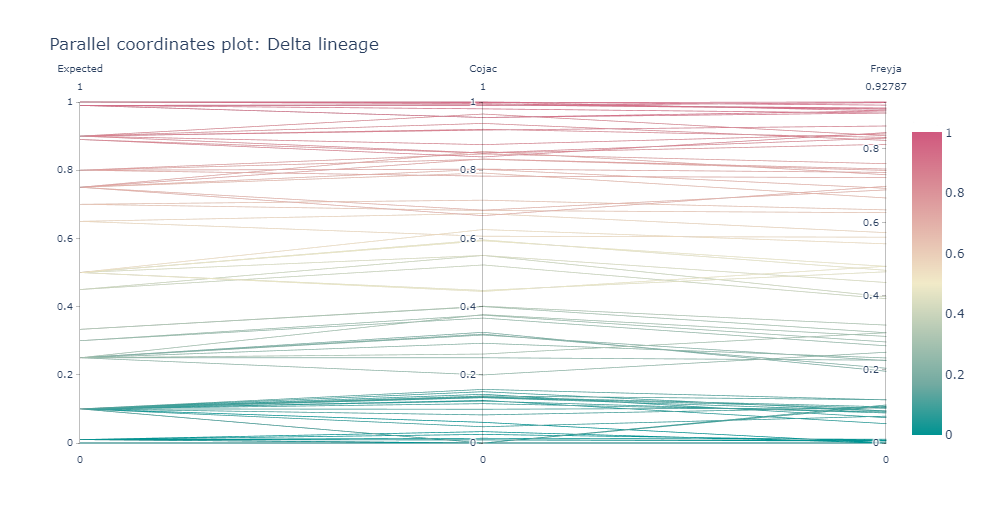
\includegraphics[width=0.8\textwidth]{figures/further/pc-delta-all.png}
            \captionof{figure}{Parallel coordinates plot for all samples that compare Delta lineage proportions detected by Freyja and COJAC with each other as well as with expected proportion. Left axis represents expected proportion of Delta, middle axis represents proportion of Delta lineage detected by COJAC, while right axis represents proportion of Delta lineage detected by Freyja}
            \label{fig:further:parallel-delta-all}
        \end{figure}
        \begin{figure}[H]
        	\centering
            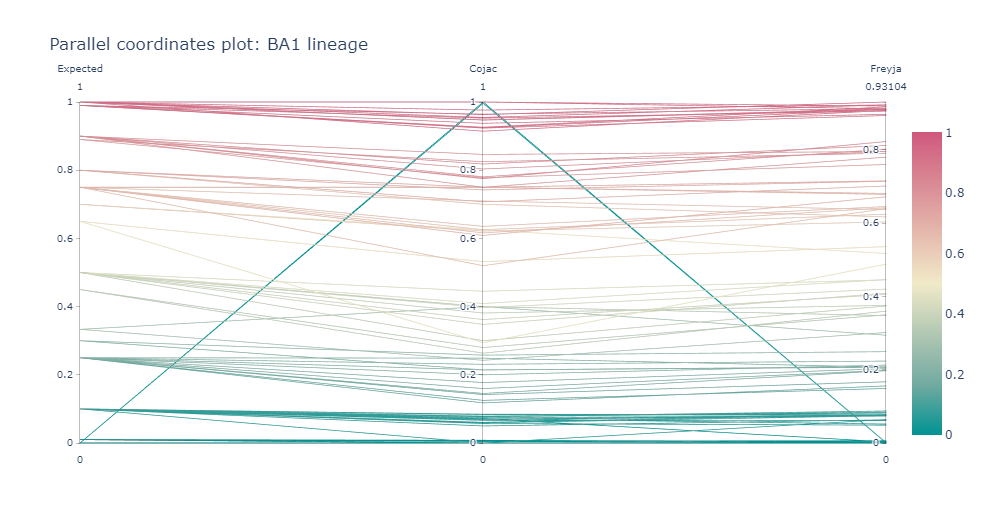
\includegraphics[width=0.8\textwidth]{figures/further/pc-ba1-all.png}
            \captionof{figure}{Parallel coordinates plot for all samples that compare BA.1 lineage proportions detected by Freyja and COJAC with each other as well as with expected proportion. Left axis represents expected proportion of BA.1, middle axis represents proportion of BA.1 lineage detected by COJAC, while right axis represents proportion of BA.1 lineage detected by Freyja}
            \label{fig:further:parallel-ba1-all}
        \end{figure}
        \begin{figure}[H]
        	\centering
            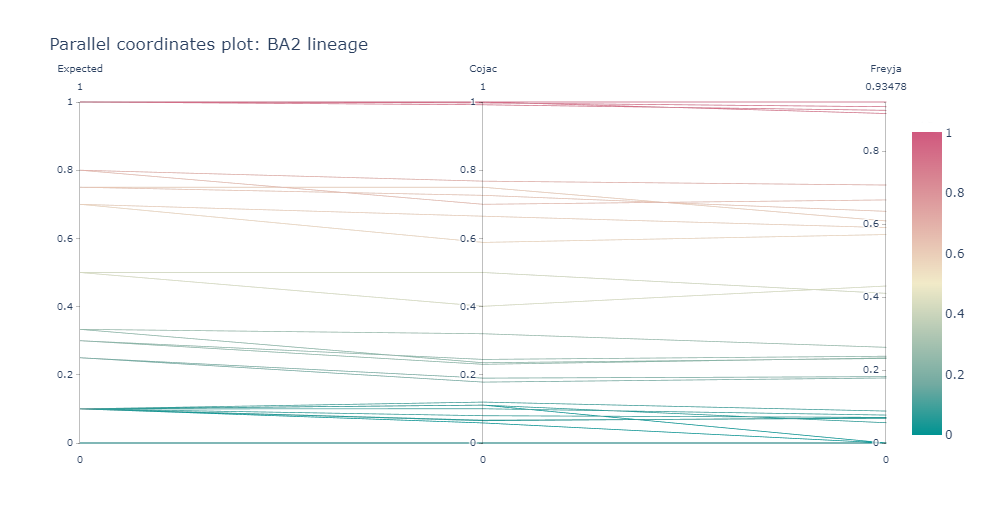
\includegraphics[width=0.8\textwidth]{figures/further/pc-ba2-all.png}
            \captionof{figure}{Parallel coordinates plot for all samples that compare BA.2 lineage proportions detected by Freyja and COJAC with each other as well as with expected proportion. Left axis represents expected proportion of BA.2, middle axis represents proportion of BA.2 lineage detected by COJAC, while right axis represents proportion of BA.2 lineage detected by Freyja}
            \label{fig:further:parallel-ba2-all}
        \end{figure}
        
        \paragraph{Parallel coordinates for mock samples with two lineages expected} \label{sec:appendix:figures:parallel-twolin}
        \Cref{fig:further:parallel-delta-twolin}, \cref{fig:further:parallel-ba1-twolin} and \cref{fig:further:parallel-ba2-twolin} depict parallel coordinates for "two lineages" group of samples considering only detection of Delta, BA.1, and BA.2 lineage respectively by Freyja and COJAC. Although, for the "two lineages" group of samples, it is not that reasonable to separate graphs into different lineages but focus on the ratio between two expected lineages. Even though, detected proportion of certain expected lineage was worthwhile to to have a look at. Thus, parallel coordinates graphs were generated in the way of one graph per lineage.
        \begin{figure}[H]
        	\centering
            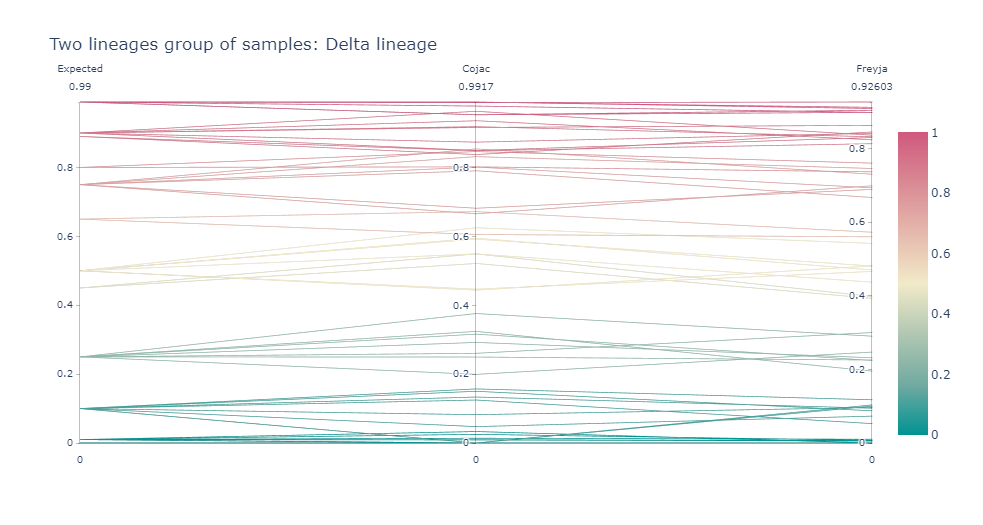
\includegraphics[width=0.8\textwidth]{figures/further/pc-twolin-delta.png}
            \captionof{figure}{Parallel coordinates plot for "two lineages group" of samples that compare Delta lineage proportions detected by Freyja and COJAC with each other as well as with expected proportion. Left axis represents expected proportion of Delta, middle axis represents proportion of Delta lineage detected by COJAC, while right axis represents proportion of Delta lineage detected by Freyja}
            \label{fig:further:parallel-delta-twolin}
        \end{figure}
        \begin{figure}[H]
        	\centering
            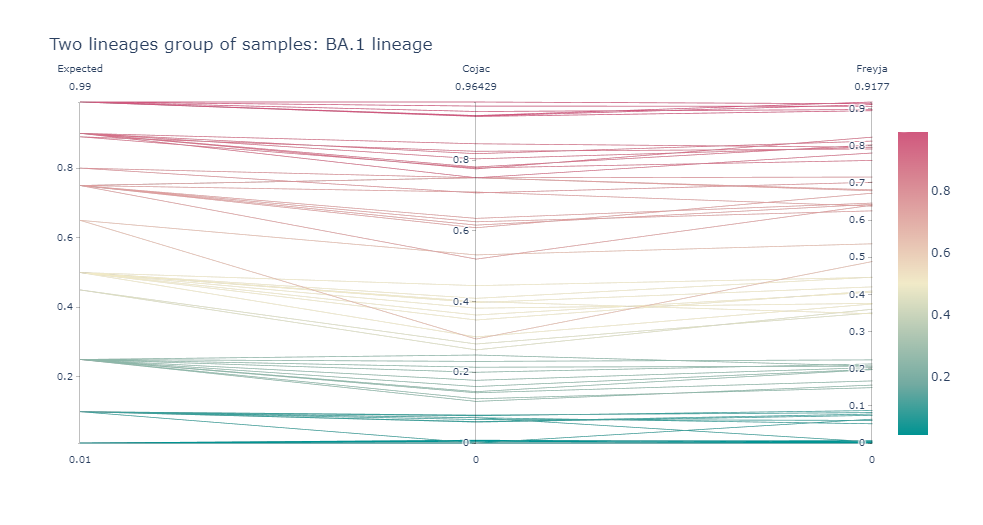
\includegraphics[width=0.8\textwidth]{figures/further/pc-twolin-ba1.png}
            \captionof{figure}{Parallel coordinates plot for "two lineages group" of samples that compare BA.1 lineage proportions detected by Freyja and COJAC with each other as well as with expected proportionfor "two lineages group" of samples. Left axis represents expected proportion of BA.1, middle axis represents proportion of BA.1 lineage detected by COJAC, while right axis represents proportion of BA.1 lineage detected by Freyja}
            \label{fig:further:parallel-ba1-twolin}
        \end{figure}
        \begin{figure}[H]
        	\centering
            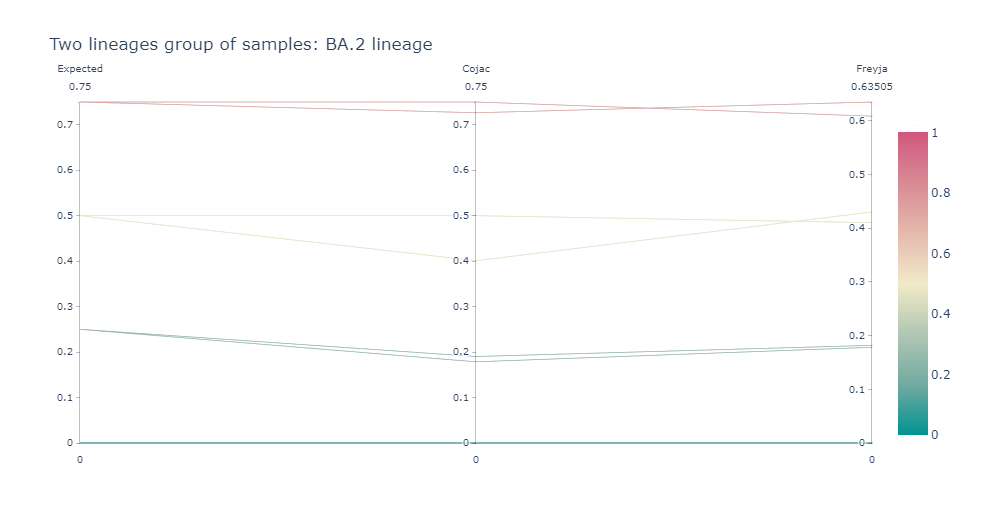
\includegraphics[width=0.8\textwidth]{figures/further/pc-twolin-ba2.png}
            \captionof{figure}{Parallel coordinates plot for "two lineages group" of samples that compare BA.2 lineage proportions detected by Freyja and COJAC with each other as well as with expected proportion for "two lineages group" of samples. Left axis represents expected proportion of BA.2, middle axis represents proportion of BA.2 lineage detected by COJAC, while right axis represents proportion of BA.2 lineage detected by Freyja}
            \label{fig:further:parallel-ba2-twolin}
        \end{figure}
        
        \subsubsection{Example of different types of plots for one mock sample} 
        \Cref{fig:further:bar-s1}, \cref{fig:further:pc-s1} and \cref{fig:further:line-s1} show plots generated per sample to make detailed observations. The example for the sample1 is provided below. However, these graphs were constructed for every sample during this master thesis. Types of plots that were generated per one sample: i) bar plot (\cref{fig:further:bar-s1}); ii) parallel coordinates plot (\cref{fig:further:pc-s1}); iii) line plot (\cref{fig:further:line-s1}), to look at absolute values of lineage proportion against scaled values in parallel coordinates. The comparison with expected lineage proportions was included in these plots.
.
        \begin{figure}[H]
        	\centering
            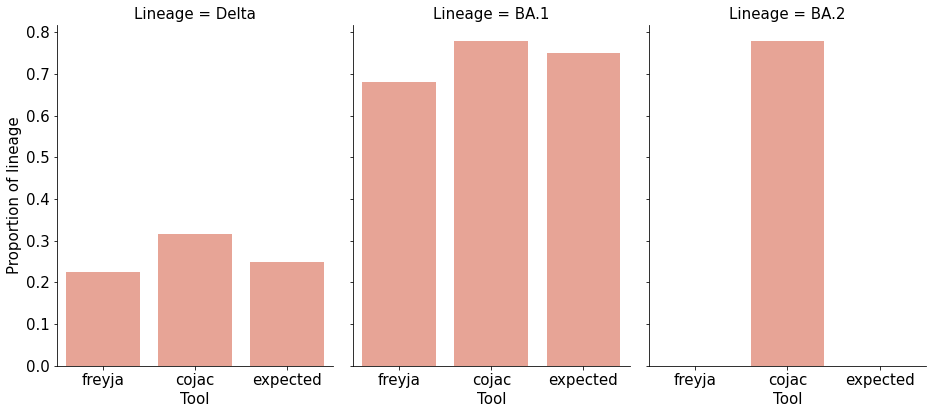
\includegraphics[width=0.8\textwidth]{figures/further/bar-s1.png}
            \captionof{figure}{Bar plot for sample 1.}
            \label{fig:further:bar-s1}
        \end{figure}
        \begin{figure}[H]
        	\centering
            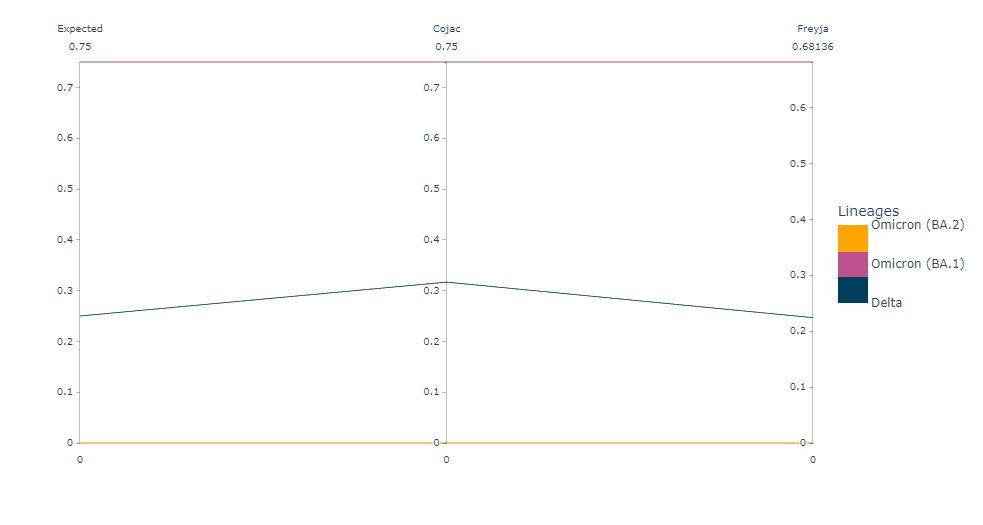
\includegraphics[width=0.8\textwidth]{figures/further/pc-s1.png}
            \captionof{figure}{Parallel coordinates plot for sample 1}
            \label{fig:further:pc-s1}
        \end{figure}
        \begin{figure}[H]
        	\centering
            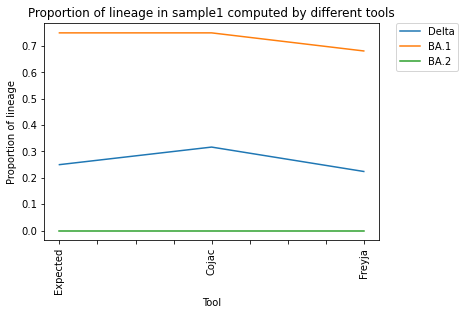
\includegraphics[width=0.8\textwidth]{figures/further/line-s1.png}
            \captionof{figure}{Line plot for sample 1}
            \label{fig:further:line-s1}
        \end{figure}
        
        \subsubsection{Collection of bar plots across all mock samples} \label{sec:appendix:figures:bars-all}
        \Cref{fig:further:bars-delta-all}, \cref{fig:further:bars-ba1-all} and \cref{fig:further:bars-ba2-all} depict barplots for all samples considering only detection of Delta, BA.1, and BA.2 lineage respectively.
        
        \begin{figure}[H]
        	\centering
            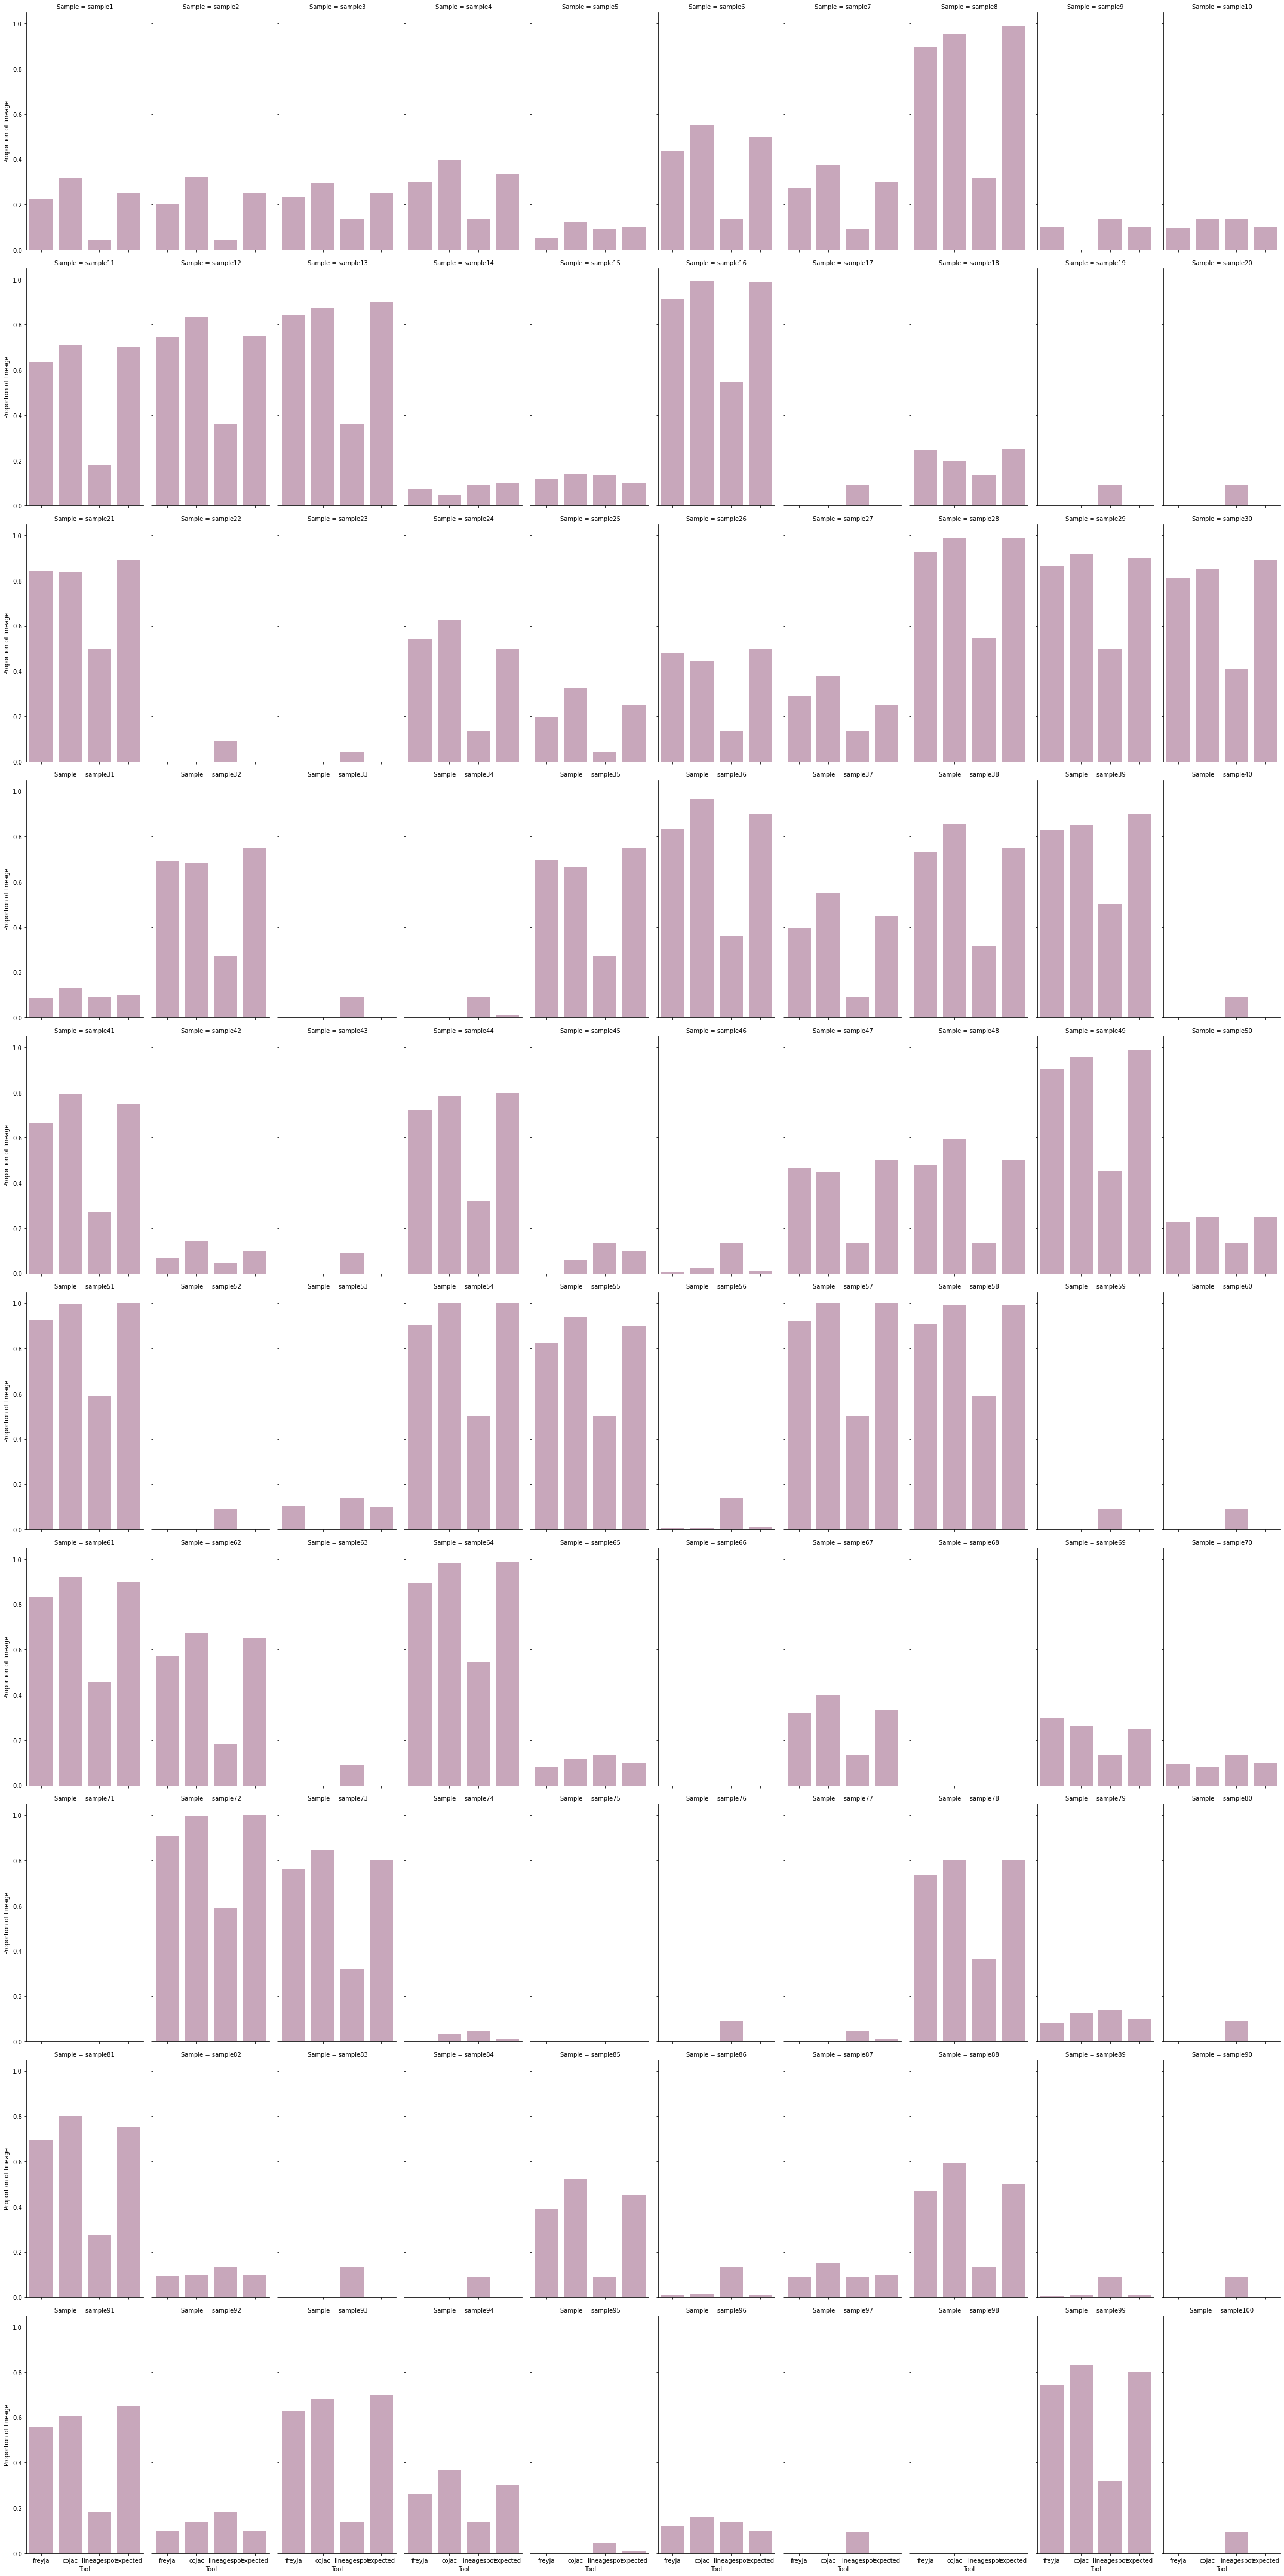
\includegraphics[width=0.7\textwidth]{figures/further/bars-delta-all.png}
            \captionof{figure}{Bar plots that compare Delta lineage proportions detected by Freyja and COJAC with each other as well as with expected proportion.}
            \label{fig:further:bars-delta-all}
        \end{figure}
        \begin{figure}[H]
        	\centering
            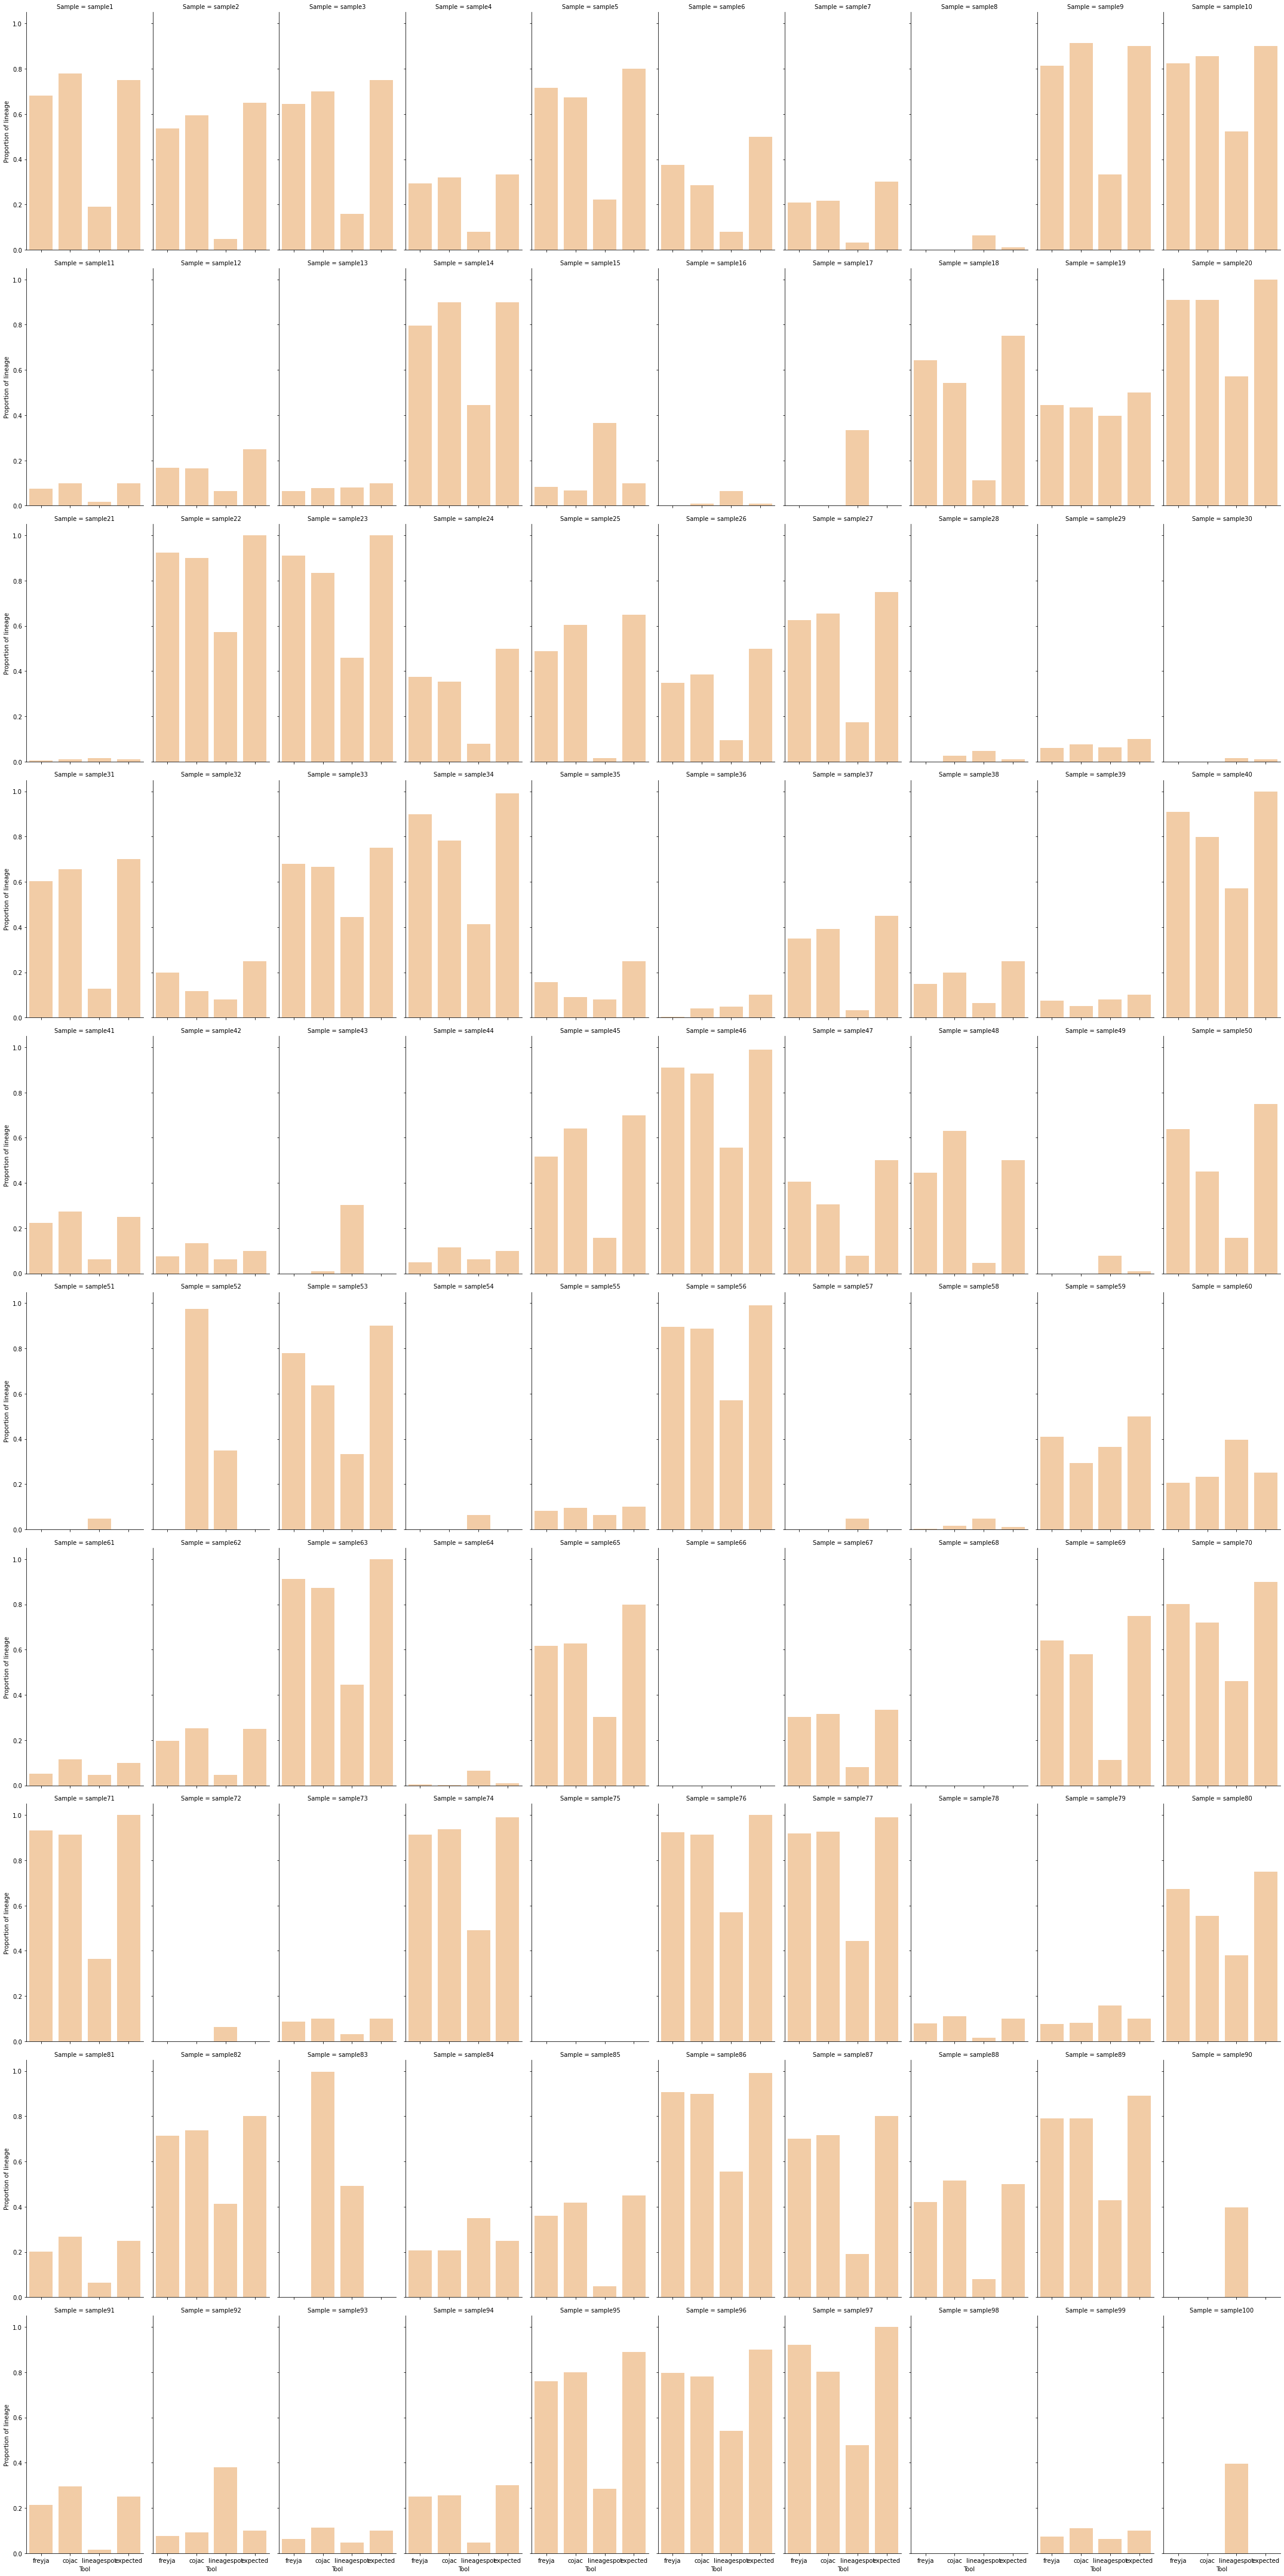
\includegraphics[width=0.7\textwidth]{figures/further/bars-ba1-all.png}
            \captionof{figure}{Bar plots that compare BA.1 lineage proportions detected by Freyja and COJAC with each other as well as with expected proportion}
            \label{fig:further:bars-ba1-all}
        \end{figure}
        \begin{figure}[H]
        	\centering
            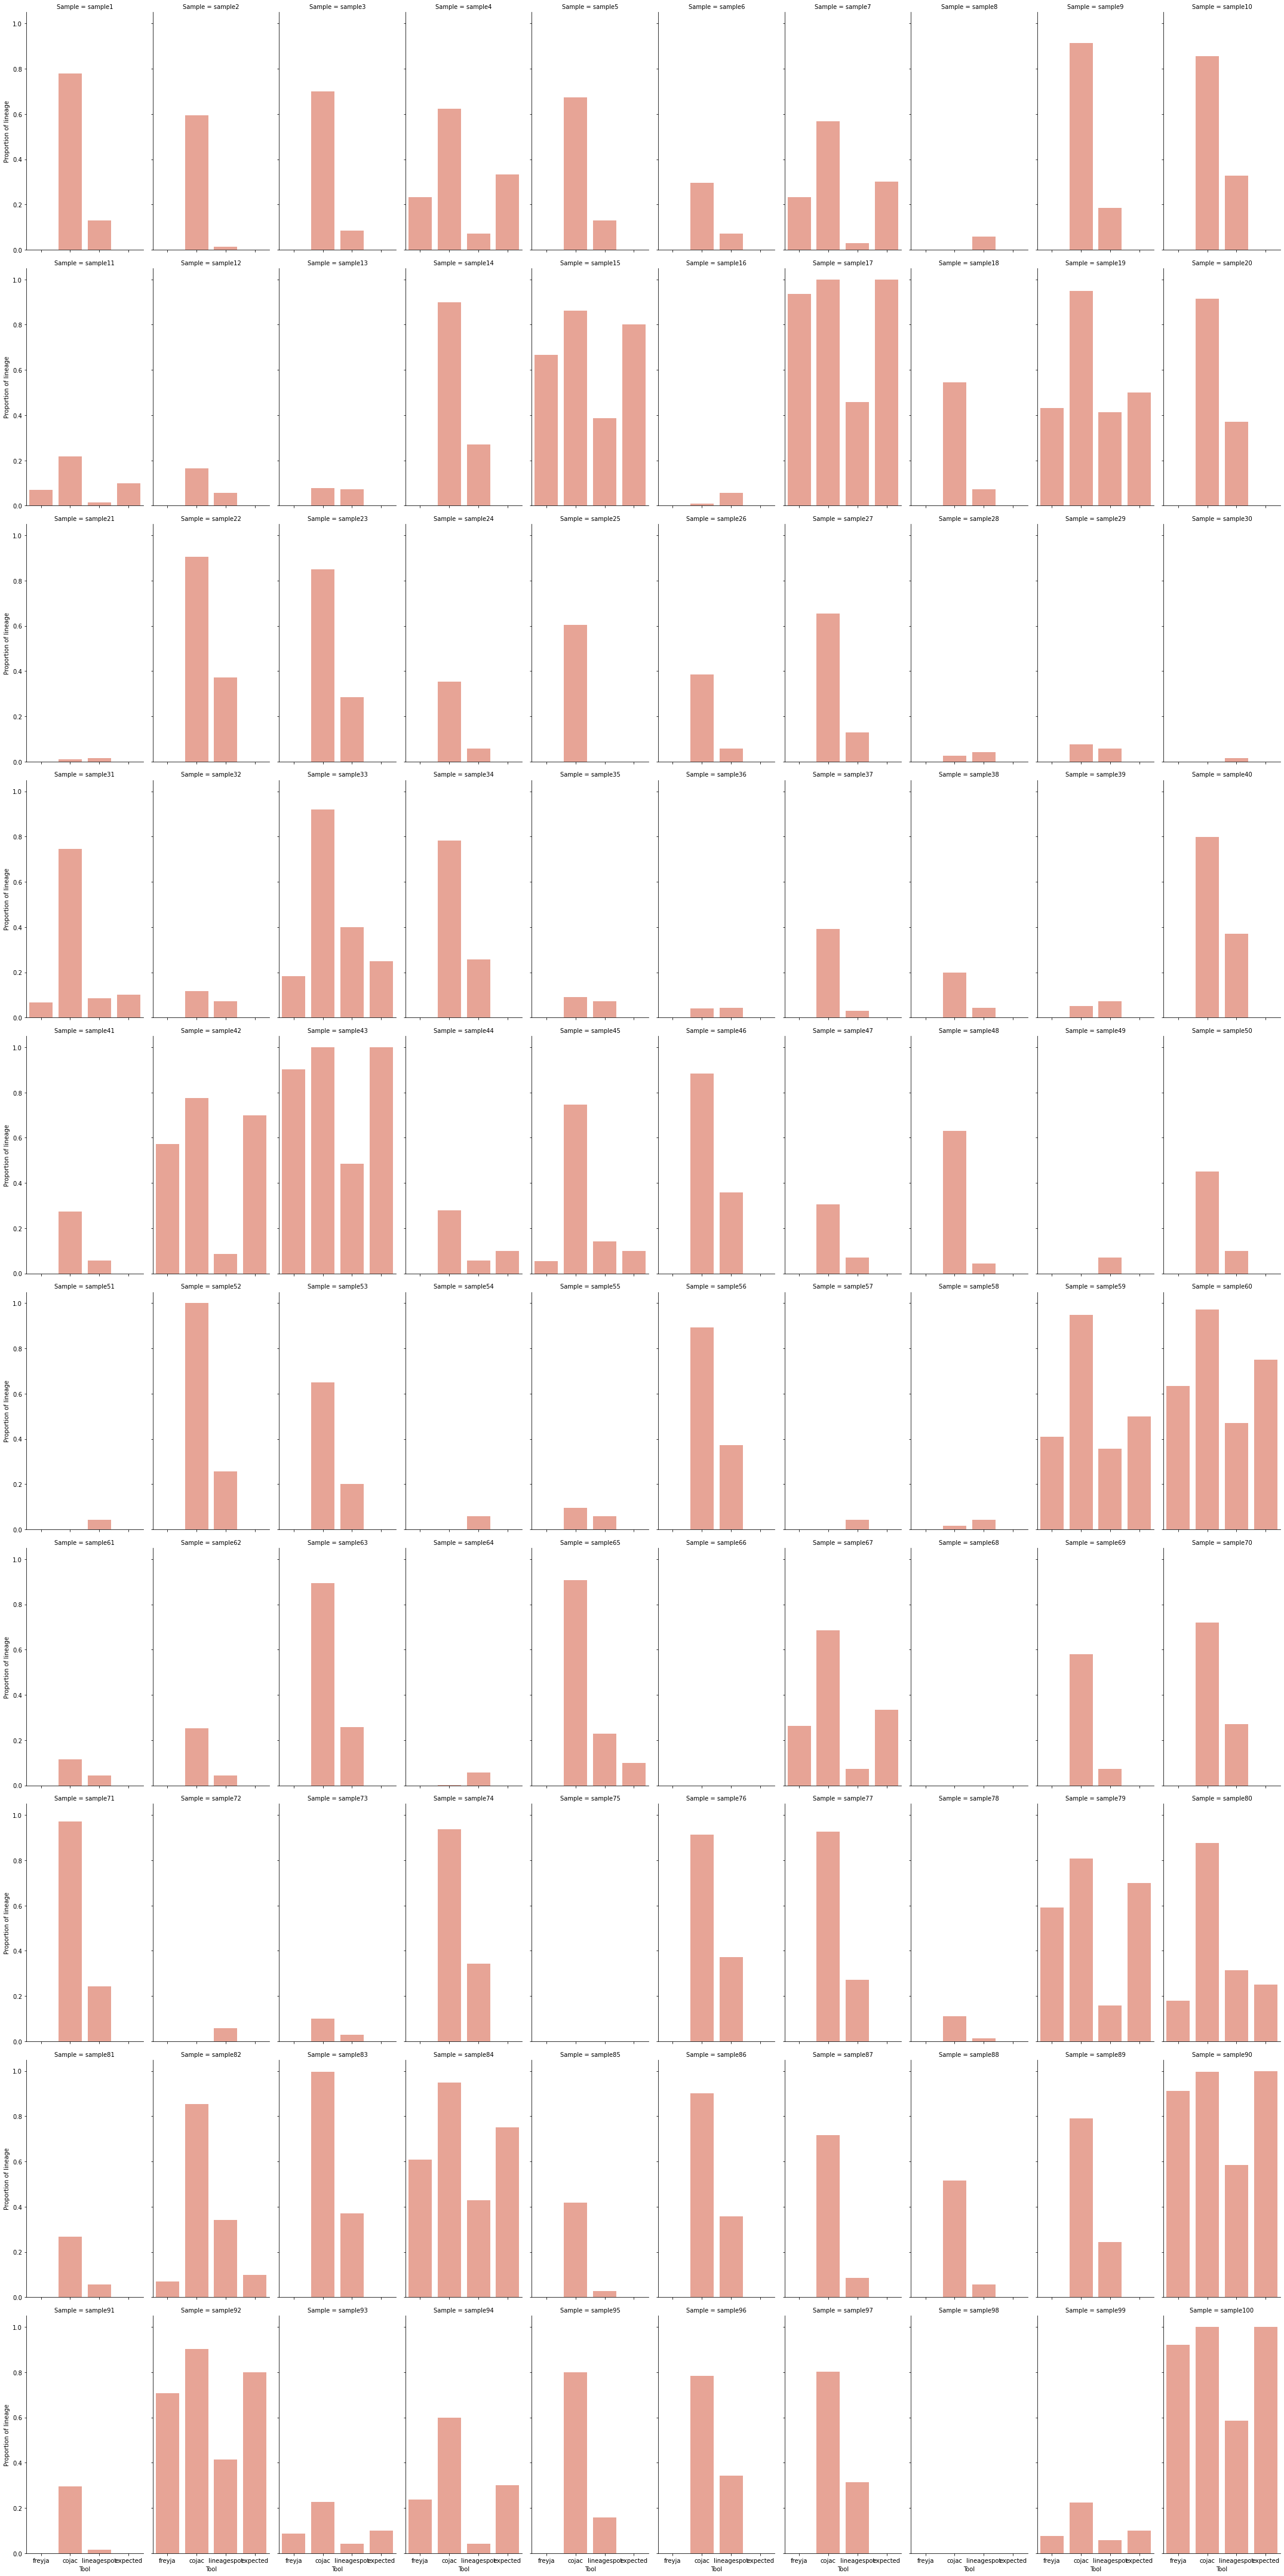
\includegraphics[width=0.7\textwidth]{figures/further/bars-ba2-all.png}
            \captionof{figure}{Bar plots that compare BA.2 lineage proportions detected by Freyja and COJAC with each other as well as with expected proportion.}
            \label{fig:further:bars-ba2-all}
        \end{figure}
        
       \subsubsection{Distribution of lineages proportions detected by Lineagespot across all mock samples}  
        \Cref{fig:further:dist-ls} represents the proportions of every lineage detected by Lineagespot on mock dataset. Observed that most of the samples, more than 50\%, according to Lineagespot, carry a small proportion, no more than 0.15, of lineage abundance, while higher proportions of all 3 lineages are present in less amount of samples.
        \begin{figure}[H]
        	\centering
            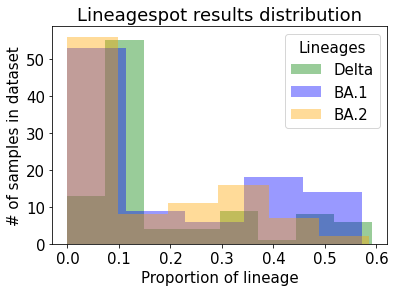
\includegraphics[width=0.5\textwidth]{figures/further/distr-lineagespot.png}
            \captionof{figure}{All three considered lineages (Delta, BA.1, BA.2) proportion distribution among results detected by Lineagespot on mock dataset.}
            \label{fig:further:dist-ls}
        \end{figure}
        
    \subsection{Supplementary tables}
        \subsubsection{Freyja aggregated demixed data} \label{sec:appendix:tabs:freyja}
\begin{landscape}
            \centering\vspace*{\fill}
                \begin{table}[ht!]
                \tiny
                \begin{tabular}{l|l|l|l|l|l}
                            &summarized&lineages&abundances&resid&coverage\\ \hline
                SRR12596165.fastq&"[('Other', 0.9999999999972105)]"&\multicolumn{1}{m{5cm}|}{B.10 B.47 B.23 B.26 B.1.14 B.20 B}&\multicolumn{1}{m{5cm}|}{0.14285714 0.14285714 0.14285714 0.14285714 0.14285714 0.14285714 0.14285714}&2.63E-12&1.926550271\\ \hline
                SRR12596166.fastq&"[('Other', 0.9999999999983175)]"&\multicolumn{1}{m{5cm}|}{B.1.1.174 B.10 B.47 B.23 B.26 B.1.14 B.20 B}&\multicolumn{1}{m{5cm}|}{0.55555600 0.06349200 0.06349200 0.06349200 0.06349200 0.06349200 0.06349200 0.06349200}&1.162673375&1.926550271\\ \hline
                SRR12596167.fastq&"[('Other', 0.9999999999996593)]"&\multicolumn{1}{m{5cm}|}{B.10 B.47 B.23 B.26 B.1.14 B.20 B}&\multicolumn{1}{m{5cm}|}{0.14285714 0.14285714 0.14285714 0.14285714 0.14285714 0.14285714 0.14285714}&0.75&1.926550271\\ \hline
                SRR12596168.fastq&"[('Other', 0.9999999999582964)]"&\multicolumn{1}{m{5cm}|}{B.1.1.174 B.1.1.161 B.1.564 B.1.12 B.1.607 B.1.413 B.1.324 B.1.453 B.1.1.372 B.1.1 B.1.1.92 B.1.1.294 B.1.1.180 B.1.1.43 B.1.1.59 B.1.1.463 B.1.1.402 B.1.1.10 B.1.1.208 B.1.1.61 B.10 B.47 B.23 B.26 B.1.14 B.20 B}&\multicolumn{1}{m{5cm}|}{0.27027000 0.08080800 0.05555550 0.05555550 0.05555550 0.05555550 0.05555550 0.05555550 0.02377383 0.02377383 0.02377383 0.02377383 0.02377383 0.02377383 0.02377383 0.02377383 0.02377383 0.02377383 0.02377383 0.02377383 0.00432900 0.00432900 0.00432900 0.00432900 0.00432900 0.00432900 0.00432900}&0.4968557797&1.926550271\\ \hline
                SRR12596169.fastq&"[('Other', 0.9999999999979102)]"&\multicolumn{1}{m{5cm}|}{B.1.111 B.1.1.174 B.1.479 B.1.22 B.1.533 B.1.12 B.1.607 B.1.453 B.1.324 B.1.413 B.1.564 B.1.199 B.1.378 B.1.201 B.1.215 B.1}&\multicolumn{1}{m{5cm}|}{0.14432305 0.14285700 0.09853229 0.06999717 0.05158700 0.04640292 0.04640292 0.04640292 0.04640292 0.04640292 0.04640292 0.04285720 0.04285720 0.04285720 0.04285720 0.04285720}&0.7140985235&1.926550271\\ \hline
                SRR12596170.fastq&"[('Other', 0.9999999999987905)]"&\multicolumn{1}{m{5cm}|}{B.1.533 B.1.370 B.1.301 B.1.424 B.1.111 B.1.479 B.1.201 B.1.378 B.1.199 B.1.215 B.1 B.1.22 B.1.453 B.1.324 B.1.413 B.1.607 B.1.12 B.1.564 B.1.1.161 B.10 B.47 B.23 B.26 B.1.14 B.20 B}&\multicolumn{1}{m{5cm}|}{0.15773800 0.11717199 0.11641401 0.11641400 0.05154872 0.03906387 0.03904760 0.03904760 0.03904760 0.03904760 0.03904760 0.03189755 0.01718081 0.01718081 0.01718081 0.01718081 0.01718081 0.01718081 0.00892900 0.00892857 0.00892857 0.00892857 0.00892857 0.00892857 0.00892857 0.00892857}&0.4778312073&1.926550271\\ \hline
                SRR12596171.fastq&"[('Other', 0.9979179208943117)]"&\multicolumn{1}{m{5cm}|}{B.1.509 B.1.12 B.1.607 B.1.453 B.1.324 B.1.413 B.1.564 B.10 B.47 B.23 B.26 B.1.14 B.20 B}&\multicolumn{1}{m{5cm}|}{0.87096800 0.01560282 0.01560282 0.01560282 0.01560282 0.01560282 0.01560282 0.00476186 0.00476186 0.00476186 0.00476186 0.00476186 0.00476186 0.00476186}&0.3834278298&1.926550271\\ \hline
                SRR12596172.fastq&"[('Other', 0.9999999999983878)]"&\multicolumn{1}{m{5cm}|}{B.1.301 B.1.424 B.1.370 B.1.1.174 B.1.453 B.1.12 B.1.607 B.1.324 B.1.413 B.1.564 B.47 B.20 B.1.14 B.26 B.23 B B.10 B.1.533 B.1.111 B.1.22 B.1.479}&\multicolumn{1}{m{5cm}|}{0.27497564 0.27497564 0.27312572 0.03731300 0.01588226 0.01588226 0.01588226 0.01588226 0.01588226 0.01588226 0.00529100 0.00529100 0.00529100 0.00529100 0.00529100 0.00529100 0.00529100 0.00367100 0.00125773 0.00118732 0.00116342}&0.54272957&1.926550271\\ \hline
                SRR12596173.fastq&"[('Other', 0.9999999999972105)]"&\multicolumn{1}{m{5cm}|}{B.10 B.47 B.23 B.26 B.1.14 B.20 B}&\multicolumn{1}{m{5cm}|}{0.14285714 0.14285714 0.14285714 0.14285714 0.14285714 0.14285714 0.14285714}&2.63E-12&1.926550271\\ \hline
                SRR12596174.fastq&"[('Other', 0.999999999979265)]"&\multicolumn{1}{m{5cm}|}{B.1.509 B.1.2 B.1.370 B.1.301 B.1.424 B.1.324 B.1.564 B.1.413 B.1.453 B.1.607 B.1.12 B.1.596 B.47 B.20 B.1.14 B.26 B.23 B B.10 B.1 B.1.215 B.1.201 B.1.378 B.1.199}&\multicolumn{1}{m{5cm}|}{0.28000000 0.20118712 0.06037074 0.06035913 0.06035913 0.04567167 0.04567167 0.04567167 0.04567167 0.04567167 0.04567167 0.02797988 0.00432900 0.00432900 0.00432900 0.00432900 0.00432900 0.00432900 0.00432900 0.00108220 0.00108220 0.00108220 0.00108220 0.00108220}&0.8515939213&1.926550271\\ \hline
                SRR12596175.fastq&"[('Other', 0.9905735237538151)]"&\multicolumn{1}{m{5cm}|}{B.1.509 B.1.2 B.1.382 B.1.111 B.10 B.47 B.23 B.26 B.1.14 B.20 B B.1.479 B.1.22}&\multicolumn{1}{m{5cm}|}{0.68478300 0.27368400 0.00451200 0.00294756 0.00294557 0.00294557 0.00294557 0.00294557 0.00294557 0.00294557 0.00294557 0.00245515 0.00157281}&0.2451972591&1.926550271\\ \hline
                \end{tabular}
                \caption{Aggregated table for Californian real-world dataset (PRJNA661613) - output of 'Freyja: aggregate' tool that aggregate demixed data for all samples in dataset} \label{tab:appendix:freyja}
                \end{table}
                \vfill
            \end{landscape}
        
        
\clearpage

